\documentclass[10pt,twocolumn]{article}
\usepackage[margin=0.70in,top=0.76in,bottom=0.80in,columnsep=0.25in]{geometry}
\usepackage{booktabs}
\usepackage{amsmath,amssymb,amsfonts}
\usepackage{graphicx}
\usepackage{hyperref}
\usepackage{xcolor}
\usepackage{multirow}
\usepackage{natbib}
\usepackage{caption}
\usepackage{microtype}
\usepackage{array}

\definecolor{linkblue}{HTML}{1D4ED8}
\definecolor{citegreen}{HTML}{047857}
\hypersetup{
    colorlinks=true,
    linkcolor=linkblue,
    citecolor=citegreen,
    urlcolor=linkblue
}

\captionsetup{font=small,labelfont=bf}
\setlength{\parskip}{1.2pt}
\setlength{\bibsep}{3.0pt}
\emergencystretch=1.5em

\title{\Large \textbf{FastBrain-9B: Selective Dual-Teacher Routing, Co-Adapted Adapter-Head Interpolation, and Request-Time Schema Post-Processing for Single-Pass Structured Decision Models}}

\author{
  \textbf{Yang Xiang} \\
  \texttt{xyxsw2021@gmail.com} \\
  {\small Model Weights (\texttt{bfloat16} \& GGUF): \url{https://huggingface.co/TypeScript/FastBrain-9B}} \\
  {\small Training Corpus: \url{https://huggingface.co/datasets/TypeScript/FastBrain-Instruct}}
}

\date{}

\begin{document}

\twocolumn[
\begin{@twocolumnfalse}
\maketitle
\vspace{-0.48cm}
\begin{abstract}
\noindent Single-pass ``System-1'' structured decision models score typed schema questions (\texttt{choice}, \texttt{noul}, and \texttt{score}) jointly in a single forward prefill pass with zero generated tokens. Although compact 9B-class decision models such as \texttt{Clef-flash} (9.41B parameters) achieve high accuracy on closed-world function verification, they exhibit pronounced miscalibration on boundary-sensitive governance tasks, including out-of-scope (OOS) intent rejection (66.63\% Macro-F1 on CLINC150+OOS caused by a 39.82\% known-intent false rejection rate under same-harness evaluation; 66.77\% in the published leaderboard snapshot), tool-calling abstention and clarification (65.39\% same-harness / 65.58\% published on When2Call), and multi-probe phishing detection (75.00\% same-harness / 71.95\% published on PhishNChips). Uniform multi-task supervised fine-tuning sharpens these decision boundaries while inducing cross-task regressions on multi-tool selection catalogs such as API-Bank ($-1.77$\,pp) and stateful environment simulation ($-3.41$\,pp). Here we present \textbf{FastBrain-9B}, a 9.41B-parameter single-pass decision model built upon a 32-layer hybrid Gated DeltaNet and full-attention backbone (\texttt{Qwen3.5-9B}) coupled with a 116.1M-parameter \texttt{JointSchemaHead}. FastBrain-9B combines three technical components: (1) selective dual-teacher Kullback--Leibler (KL) routing, which partitions training tasks between a frozen anchor teacher that preserves tool-selection and candidate-ranking distributions and a boundary-calibrated governance teacher trained with pairwise hinge margins; (2) co-adapted parameter interpolation across all 104 adapted backbone projection modules (208 low-rank adaptation factor matrices) and all 122 \texttt{JointSchemaHead} tensors, materialized in-place into the backbone and head checkpoints at zero runtime overhead; and (3) request-time schema-topology extraction paired with validation-tuned role-conditioned decision offsets, two-probe verdict averaging, and confidence-gated specialist routing. Evaluated across all 22,427 requests of the ten-benchmark Cloudflare Decision Index (v0.2.1) shortlist after 10-gram decontamination, FastBrain-9B raises the unweighted ten-benchmark mean from 74.89\% to \textbf{80.55\%} ($+5.66$\,pp same-harness; $+5.59$\,pp vs.\ the 74.96\% leaderboard snapshot), ranks first among all evaluated 9B-class models (9.0B--9.41B) across all 10 benchmarks (including ties on BFCL and ToolRet), and surpasses the 27.0B dense model \texttt{Jev} (80.32\%). On external out-of-domain community benchmarks, FastBrain-9B achieves \textbf{97.4\% balanced accuracy} ($94.9\%$ distilled raw head) and \textbf{85.1\% 7-way category Macro-F1} on \texttt{harness-hub/safeagents-judge-bench} ($562$ agent tool calls; $\#1/9$ overall), and achieves \textbf{75.25\% / 76.25\% zero-shot accuracy} ($0.1508$ KL, $0.0795$ Brier; officially ranked $\#7/42$ overall and $\#1$ among all Clef-architecture models on \texttt{LocalLLaMA/typed-decisions}, rising to $77.35\%$ with Ordinal-KL distillation and $79.70\% / 80.70\%$ when fitted on \texttt{train}). Finally, fusing $O(1)$ prefix-sum span pooling (\texttt{torch.cumsum}) with packed variable-length FlashAttention accelerates \texttt{JointSchemaHead} execution by $1.90\times$ ($3.27\,\text{ms} \to 1.72\,\text{ms}$), enabling sub-100\,ms serving across \texttt{SGLang} (\texttt{dev-clef}, up to $19{,}319\,\text{tok/s}$), \texttt{llama.cpp} (\texttt{b11430} GGUF \texttt{Q8\_0}/\texttt{Q4\_K\_M}, $99.86\%$ Top-1 agreement), and PyTorch on a single NVIDIA RTX PRO 6000 Blackwell GPU.
\end{abstract}
\vspace{0.30cm}
\end{@twocolumnfalse}
]

\begin{figure*}[t]
\centering
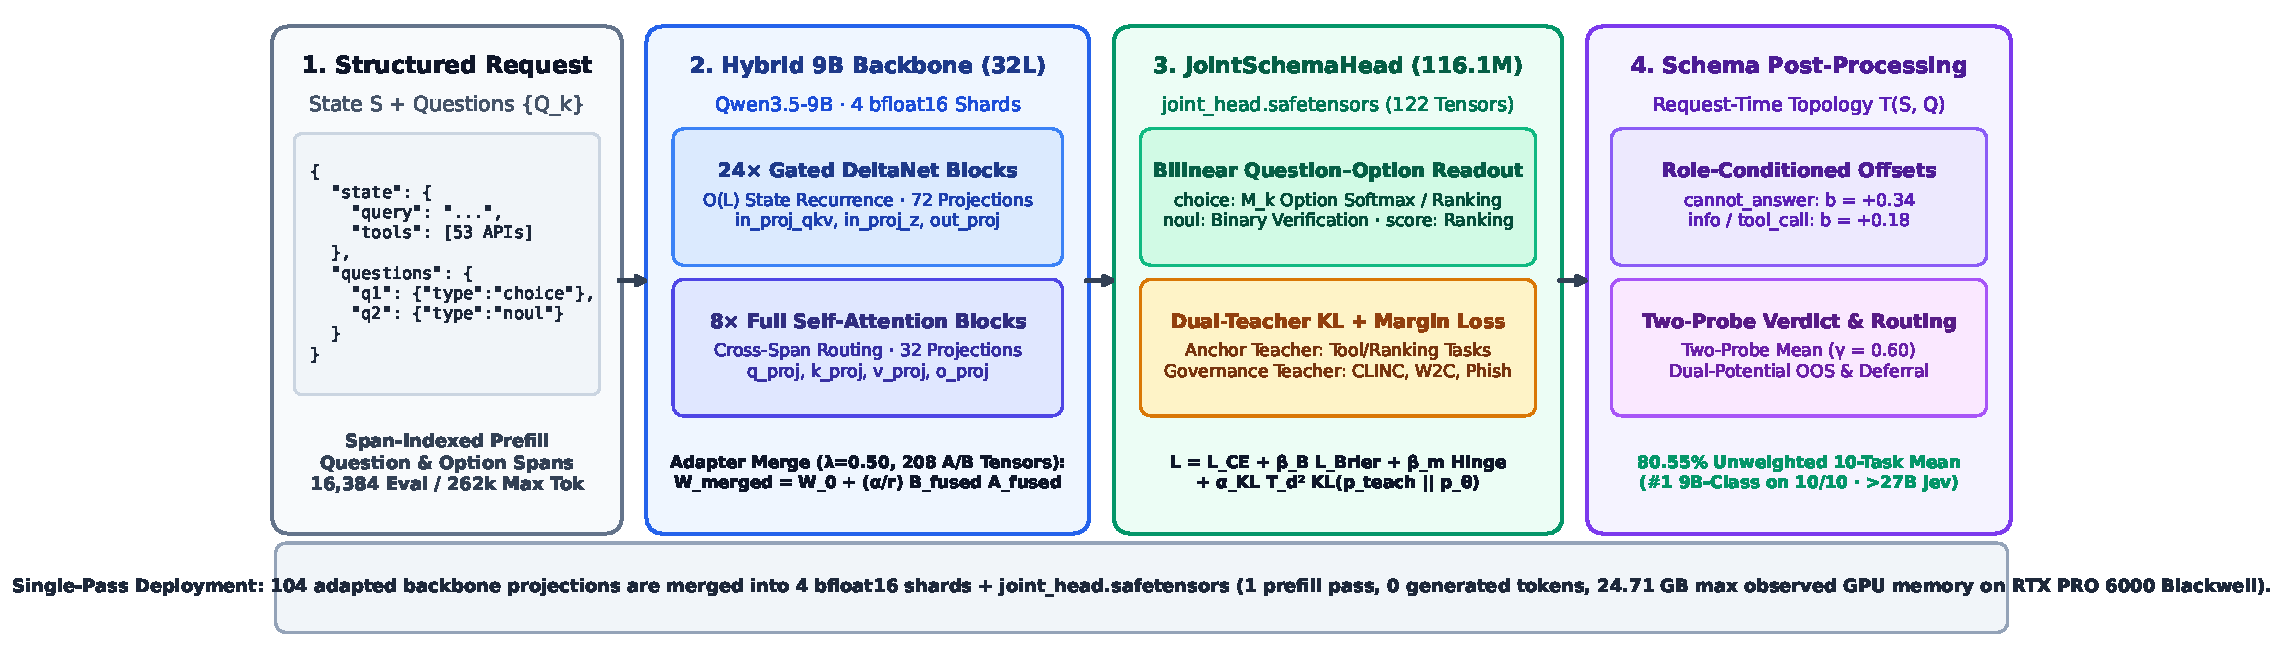
\includegraphics[width=\textwidth]{figures/fig1_architecture_pipeline.pdf}
\caption{\textbf{Architecture and three-stage training, merging, and post-processing pipeline of FastBrain-9B.} Given a structured JSON state $S$ and $K$ typed questions $\{Q_k\}_{k=1}^K$ (\texttt{choice}, \texttt{noul}, or \texttt{score}), the 32-layer hybrid \texttt{Qwen3.5-9B} backbone (24 linear-complexity Gated DeltaNet blocks and 8 full self-attention blocks) encodes the prompt and candidate option spans in a single prefill pass with zero generated tokens. During training, selective dual-teacher KL routing and pairwise hinge margins prevent cross-task interference between 53-tool API catalogs and boundary-governance tasks. All 104 adapted backbone projection modules (208 LoRA $A/B$ factor matrices) and 122 \texttt{JointSchemaHead} tensors are interpolated in weight space ($\lambda=0.50$) and materialized into four \texttt{bfloat16} backbone shards plus \texttt{joint\_head.safetensors}, followed by request-time schema-topology extraction $T(S, Q)$ and task-family post-processing.}
\label{fig:architecture}
\end{figure*}

\section{Introduction}
Production agentic pipelines, enterprise API gateways, and real-time security filters execute thousands of structured control decisions per second: selecting which function signature to invoke from a large tool registry \citep{patil2024gorilla,li2023apibank}, determining when to abstain or request user clarification if required arguments are missing \citep{ross2025when2call}, rejecting out-of-scope (OOS) queries across fine-grained intent taxonomies \citep{larson2019clinc150,casanueva2020banking77}, and reranking candidate tools or evidence passages \citep{shi2025toolret,su2025bright,reddy2022esci}. Standard autoregressive language models execute these routing decisions by sequentially decoding dozens of formatting and JSON schema tokens. Sequential token generation incurs multi-hundred-millisecond tail latencies, requires constrained decoding to guarantee valid syntax, and produces poorly calibrated token-level probabilities \citep{guo2017calibration}.

Single-pass ``System-1'' structured decision architectures---including \texttt{Clef} (27.36B parameters), \texttt{Clef-flash} (9.41B), \texttt{Jev} (27.0B), \texttt{Kev 9B} (9.0B), and \texttt{Laya} (0.42B) \citep{cloudflare2026clef,apolinario2026decisionindex}---eliminate autoregressive decoding by coupling a long-context hybrid backbone \citep{yang2024deltanet,yang2025gateddeltanet} with a discriminative \texttt{JointSchemaHead}. By encoding the input state and all candidate option spans into a single prompt and pooling span representations from the final hidden states, these models score multiple-choice (\texttt{choice}), binary verification (\texttt{noul}), and candidate ranking (\texttt{score}) questions in one forward prefill pass with zero output tokens. While the 9.41B-parameter \texttt{Clef-flash} checkpoint matches larger models on closed-world function calling (98.76\% on BFCL), our diagnostic evaluation across the 22,427-request ten-benchmark Decision Index (v0.2.1) shortlist \citep{apolinario2026decisionindex} demonstrates that 9B-class single-pass models experience severe boundary miscalibration when candidate options represent asymmetric epistemic actions (such as abstention vs.\ execution or open-set rejection vs.\ in-scope classification).

Specifically, we characterize three interacting failure mechanisms in 9B-class single-pass decision models. First, on high-cardinality open-set intent classification (CLINC150+OOS; \citealp{larson2019clinc150}), \texttt{Clef-flash} assigns an elevated logit to the catch-all \texttt{out\_of\_scope} option (\texttt{option\_80}) whenever probability mass is divided among semantically adjacent banking or utility intents; under controlled same-harness evaluation, it falsely rejects $1{,}792$ of $4{,}500$ legitimate in-scope user requests (39.82\% false rejection rate), reducing 151-class Macro-F1 to 66.63\% (66.77\% in the published leaderboard snapshot). Second, on four-way tool-calling governance (When2Call; \citealp{ross2025when2call}), \texttt{Clef-flash} exhibits strong prior bias toward direct answering and immediate tool execution: it predicts direct prose answers on 33.82\% ($438/1{,}295$) of queries where no compatible tool exists (\texttt{cannot\_answer} recall of 40.46\%) and invokes tools with fabricated arguments on 19.87\% ($211/1{,}062$) of underspecified requests that require user clarification (\texttt{request\_for\_info}). Third, optimizing these decision boundaries via uniform multi-task supervised fine-tuning (SFT) or single-teacher distillation induces cross-task representation drift \citep{ilharco2023taskarithmetic,yadav2023ties}: gradient updates that sharpen abstention and OOS boundaries perturb the bilinear span representations of the 53-tool API-Bank catalog \citep{li2023apibank} and multi-step state simulation schemas, lowering API-Bank accuracy by $1.77$\,pp and Home Appliances accuracy by $3.41$\,pp.

To resolve this stability--plasticity trade-off in single-pass decision models, we coordinate task-routed distillation during training, co-adapted parameter interpolation across the backbone and schema head after training, and request-time schema-dependent post-processing at inference. We introduce \textbf{FastBrain-9B} (9.41B total parameters), which adapts all 104 linear-attention and full-attention projection modules of the 32-layer \texttt{Qwen3.5-9B} hybrid backbone alongside all 122 tensors of the 116.1M-parameter \texttt{JointSchemaHead} (Figure~\ref{fig:architecture}). Combining selective dual-teacher KL routing, co-adapted LoRA-and-head interpolation folded into the \texttt{bfloat16} checkpoint, and request-time schema post-processing, FastBrain-9B reaches an \textbf{80.55\%} unweighted ten-benchmark mean across the 22,427-request Decision Index shortlist. Across all eight classification benchmarks ($N = 21{,}522$), it corrects $2{,}763$ erroneous base-model predictions against $99$ new errors (net $+2{,}664$ requests; $+2{,}666$ across the seven non-ESCI classification tasks) with zero new errors on BFCL, API-Bank, and Home Appliances, ranks first among all evaluated 9B-class models across all 10 benchmarks, and exceeds the 27.0B dense model \texttt{Jev} (80.32\%) at one-third the parameter count.

\section{Related Work}

\subsection{Tool-Calling Governance and Retrieval}
Early evaluations of tool-augmented language models focused on syntactic validity and argument matching under closed-world assumptions, where a relevant API is guaranteed to exist in the prompt. Gorilla and the Berkeley Function Calling Leaderboard (BFCL; \citealp{patil2024gorilla}) established abstract syntax tree (AST) sub-tree verification across Python, Java, and REST APIs, while API-Bank \citep{li2023apibank} evaluated multi-turn planning, retrieval, and invocation across 53 API tools. As tool registries scaled to thousands of heterogeneous specifications, ToolRet \citep{shi2025toolret} showed that dense retrievers struggle to align user instructions with complex tool documentation, and BRIGHT \citep{su2025bright} demonstrated that reasoning-intensive retrieval requires logical and mathematical deduction beyond lexical overlap. Extending beyond closed-world invocation, \citet{ross2025when2call} introduced When2Call to evaluate whether models know when to abstain from calling a tool, formalizing a four-way governance taxonomy: \texttt{direct}, \texttt{tool\_call}, \texttt{request\_for\_info}, and \texttt{cannot\_answer}. Whereas \citet{ross2025when2call} applied preference optimization to autoregressive generators, we address tool governance within a single-pass discriminative schema head through pairwise margin training and role-conditioned decision offsets.

\subsection{Intent Detection and Open-Set Rejection}
Fine-grained intent classification in enterprise assistants requires distinguishing dozens of overlapping domain intents while rejecting unsupported user queries. BANKING77 \citep{casanueva2020banking77} benchmarks discrimination among 77 banking intents, whereas CLINC150 \citep{larson2019clinc150} pairs 150 in-scope intents across 10 domains with 1,000 out-of-scope (OOS) evaluation utterances. Prior studies have shown that softmax classifiers trained over high-cardinality label spaces miscalibrate open-set thresholds \citep{guo2017calibration,larson2019clinc150}. In single-pass schema models where the OOS catch-all option is encoded as an explicit text span alongside 150 known intent descriptions, cross-option attention pooling creates an asymmetric logit shift toward the OOS span, which we counter via bidirectional hinge-margin training, Brier score regularization \citep{brier1950verification}, and dual-potential OOS calibration.

\subsection{Hybrid Linear Attention and Single-Pass Heads}
Standard Transformer self-attention incurs quadratic compute and linear KV-cache memory growth with sequence length \citep{dao2022flashattention}. \citet{yang2024deltanet} introduced DeltaNet, applying the delta update rule to linear transformers via hardware-efficient chunkwise parallel primitives (\texttt{chunk\_gated\_delta\_rule}), and subsequently proposed Gated Delta Networks \citep{yang2025gateddeltanet} by combining data-dependent gating with delta-rule associative memory erasure. Our \texttt{Qwen3.5-9B} backbone interleaves 24 Gated DeltaNet layers with 8 full self-attention layers (in a $3:1$ ratio across 8 macro-stages), bounding recurrent state memory in 75\% of layers while preserving exact cross-span token routing in the 8 full-attention blocks. Atop this hybrid backbone, the \texttt{JointSchemaHead} \citep{cloudflare2026clef} extracts span-pooled question and option representations to score multiple schema questions in one forward pass.

\subsection{Task Arithmetic and Parameter Interpolation}
Multi-task fine-tuning of a shared pre-trained model often degrades individual task performance due to gradient conflict \citep{ilharco2023taskarithmetic}. Model Soups \citep{wortsman2022modelsoups} showed that averaging checkpoints fine-tuned within a shared loss basin improves generalization at zero inference cost. Task Arithmetic \citep{ilharco2023taskarithmetic} formalized task vectors ($\tau_t = \theta_t - \theta_0$), while TIES-Merging \citep{yadav2023ties} and DARE \citep{yu2024dare} reduced parameter redundancy during static weight merging. For low-rank adapters \citep{hu2022lora}, LoraHub \citep{huang2024lorahub} formulated task-level composition by linearly interpolating LoRA $A$ and $B$ factor matrices prior to multiplication. We extend factor-level adapter interpolation to hybrid linear-attention backbones coupled with a 116.1M-parameter discriminative readout head, showing that co-adapted interpolation of both the 208 LoRA factor tensors and the 122 \texttt{JointSchemaHead} tensors is essential to maintain coordinate alignment across the backbone--head interface.

\section{Diagnostic Audit of Single-Pass Decision Vulnerabilities}
\label{sec:audit}

\subsection{Single-Pass Schema Formulation}
Let $x = (S, \{Q_k\}_{k=1}^K)$ denote a structured decision request comprising a JSON context state $S$ (conversation history, user query, environment state, or candidate tool definitions) and $K \ge 1$ schema questions. Each question $Q_k = (\text{type}_k, q_k, \mathcal{O}_k)$ specifies a question identifier and prompt $q_k$, a decision primitive $\text{type}_k \in \{\texttt{choice}, \texttt{noul}, \texttt{score}\}$, and a candidate option set $\mathcal{O}_k = \{o_{k,1}, \dots, o_{k,M_k}\}$ (with $M_k = 2$ implicit binary outcomes for $\texttt{noul}$). During input serialization, the processor flattens $S$ and $\{Q_k\}_{k=1}^K$ into a single token sequence of length $L$ (up to the model configuration maximum of $262{,}144$ tokens; capped at $16{,}384$ tokens during training and evaluation) while recording exact token-index intervals $I(q_k) \subset \{1,\dots,L\}$ and $I(o_{k,m}) \subset \{1,\dots,L\}$ for every question and candidate option span.

A single forward prefill pass through the 32-layer hybrid backbone $f_\theta$ maps the token sequence to final hidden states $H \in \mathbb{R}^{L \times d}$ ($d = 4096$), with zero autoregressive decoding steps ($\text{output\_tokens} = 0$). The \texttt{JointSchemaHead} $g_\phi$ pools hidden states over each span $I(q_k)$ and $I(o_{k,m})$ via gated bilinear attention and multi-layer residual projections (122 parameter tensors totaling $116{,}129{,}859$ parameters, stored in \texttt{joint\_head.safetensors}) to emit unnormalized logits $z_{k,m} \in \mathbb{R}$:
\begin{equation}
    \mathbf{z}_k = g_\phi\big(H, I(q_k), \{I(o_{k,m})\}_{m=1}^{M_k}\big) \in \mathbb{R}^{M_k}.
    \label{eq:head_forward}
\end{equation}
For $\text{type}_k = \texttt{choice}$, candidate probabilities are computed via $p_{k,m} = \exp(z_{k,m}) / \sum_{j=1}^{M_k} \exp(z_{k,j})$ and the predicted option is $\hat{m}_k = \arg\max_m p_{k,m}$. In the \texttt{apolinario/decision-index} (v0.2.1) benchmark encoding \citep{apolinario2026decisionindex}, multi-question and listwise ranking tasks are represented using coupled per-candidate questions within a single request: BFCL requests contain $K_{\text{avg}} = 2.81$ ($1\dots 37$) binary tool-verification \texttt{choice} questions ($M_k = 2$, options $\texttt{yes}/\texttt{no}$); Home Appliances requests contain $K_{\text{avg}} = 18.07$ ($17\dots 19$) device-state \texttt{choice} questions ($2 \le M_k \le 9$); and ToolRet and BRIGHT encode $K = 32$ candidate-document \texttt{choice} questions (\texttt{doc\_0} through \texttt{doc\_31}, each with $M_k = 2$ options $\texttt{yes}/\texttt{no}$) whose continuous positive probabilities $p_{k,\texttt{yes}}$ (or native $\texttt{score}$ logits) rank the 32 candidates for $\text{nDCG@10}$ evaluation. For $\text{type}_k = \texttt{noul}$ (unrestricted binary verification in PhishNChips), $g_\phi$ outputs a scalar probability $p_k \in [0, 1]$ via a logistic readout.

\subsection{Empirical Failure Taxonomy in Base 9B Models}
Evaluating the official 9.41B-parameter \texttt{Clef-flash} checkpoint across all 22,427 requests of the ten-benchmark Decision Index (v0.2.1) shortlist exposes three primary failure modes.

\paragraph{Open-Set Logit Inflation on High-Cardinality Schemas.}
In CLINC150+OOS ($n = 5{,}500$; $K = 1$, $M_1 = 151$ options comprising 150 fine-grained intents and \texttt{option\_80} designated as \texttt{out\_of\_scope}), let $z_{\text{best}}^{\text{known}} = \max_{m \ne \text{oos}} z_m$ denote the highest in-scope logit and $\Delta z_{\text{oos}} = z_{\text{best}}^{\text{known}} - z_{\text{oos}} = \log p_{\text{best}}^{\text{known}} - \log p_{\text{oos}}$ denote the known-vs.-OOS log-odds margin. Across all $4{,}500$ known-intent test requests in \texttt{Clef-flash}, the overall median log-odds margin is $+0.734$ (median probability margin $+0.150$, 25th percentile $-0.566$). However, on $1{,}792$ of the $4{,}500$ valid in-scope requests ($\text{FRR} = 39.82\%$ under same-harness evaluation), $\Delta z_{\text{oos}}$ falls below zero with a median log-odds margin of $-0.717$ (median probability margin $-0.135$). Consequently, while OOS recall reaches 99.00\% ($990/1{,}000$), known-intent accuracy drops to 55.24\% ($2{,}486/4{,}500$) and 151-class Macro-F1 falls to 66.63\% (66.77\% in the published leaderboard snapshot).

\paragraph{Action-Role Prior Skew in Tool Governance.}
In When2Call ($n = 3{,}652$), each request presents $K = 1$ question with $M_1 = 4$ candidate responses corresponding to structural action roles $\mathcal{R} = \{\texttt{direct},\allowbreak \texttt{tool\_call},\allowbreak \texttt{request\_for\_info},\allowbreak \texttt{cannot\_answer}\}$ (in the v0.2.1 evaluation split, gold targets span $1{,}295$ $\texttt{tool\_call}$, $1{,}295$ $\texttt{cannot\_answer}$, and $1{,}062$ $\texttt{request\_for\_info}$ cases, with $0$ $\texttt{direct}$ gold targets; $\texttt{direct}$ serves as a systematic distractor on every request). In \texttt{Clef-flash}, recall reaches 82.86\% on $\texttt{tool\_call}$ ($1{,}073/1{,}295$) and 74.48\% on $\texttt{request\_for\_info}$ ($791/1{,}062$), whereas $\texttt{cannot\_answer}$ recall is only 40.46\% ($524/1{,}295$): the model misclassifies $438$ unanswerable tool queries as $\texttt{direct}$ prose answers (33.82\%) and $217$ as fabricated $\texttt{tool\_call}$ invocations (16.76\%). On $\texttt{request\_for\_info}$ ($n = 1{,}062$), it prematurely triggers $\texttt{tool\_call}$ on $211$ missing-argument queries (19.87\%).

\paragraph{Multi-Probe Verdict Disagreement in Security Screening.}
In PhishNChips ($n = 2{,}000$ emails; $1{,}000$ legitimate, $1{,}000$ phishing; \citealp{anisselbd2026phishnchips}), each request queries $K = 9$ schema fields: three binary \texttt{choice} verdict questions (\texttt{verdict}, \texttt{verdict\_alt\_click}, and \texttt{verdict\_alt\_minimal}) and six binary \texttt{noul} questions (\texttt{is\_phishing} plus five forensic signal indicators). In the Decision Index v0.2.1 evaluation harness, the benchmark score is the accuracy of the primary \texttt{verdict} field, while the remaining eight fields are recorded as auxiliary unscored probes (\texttt{unscored\_fields}). In \texttt{Clef-flash}, the primary \texttt{verdict} choice disagrees with the two-probe average of \texttt{verdict\_alt\_click} and \texttt{verdict\_alt\_minimal} on 5.8\% ($58/1{,}000$) of legitimate emails, limiting legitimate-mail recall to 73.30\% and primary verdict accuracy to 75.00\% (71.95\% in the published leaderboard snapshot).

\section{Methodology}
\label{sec:method}

\subsection{Hybrid Backbone Adaptation Scope and Training Protocol}
We initialize from the official \texttt{Cloudflare/clef-flash} checkpoint (revision \texttt{8b2e5fd1}; \citealp{cloudflare2026clef}) and attach rank-$r = 8$ ($\alpha = 16$, scaling factor $\alpha / r = 2.0$, dropout $0.05$) LoRA adapters \citep{hu2022lora} across all 32 layers of the \texttt{Qwen3.5-9B} backbone while jointly unlocking all 122 parameter tensors of the \texttt{JointSchemaHead} $g_\phi$ in FP32 master precision. In the 24 Gated DeltaNet linear-attention layers \citep{yang2025gateddeltanet}, adapters are placed on the fused query-key-value projection (\texttt{in\_proj\_qkv}), gating projection (\texttt{in\_proj\_z}), and output projection (\texttt{out\_proj}), yielding $24 \times 3 = 72$ adapted linear-attention projection modules. In the 8 full self-attention layers, adapters are placed on \texttt{q\_proj}, \texttt{k\_proj}, \texttt{v\_proj}, and \texttt{o\_proj}, yielding $8 \times 4 = 32$ adapted full-attention projection modules. Across all 104 adapted projection modules ($208$ LoRA $A/B$ factor matrices totaling $7.47\text{M}$ trainable adapter parameters) and 122 head tensors ($116.13\text{M}$ trainable head parameters), $123.60\text{M}$ parameters ($1.31\%$ of the $9{,}409{,}813{,}744$ total parameters) are updated during training.

Training is performed on our public structured decision corpus (\texttt{TypeScript/FastBrain-Instruct}, $108{,}278$ training instances and $5{,}699$ held-out development validation instances). To prevent training--evaluation leakage against the 22,427 Decision Index v0.2.1 evaluation requests, we applied a two-stage decontamination filter that removed $2{,}674$ candidate records exhibiting exact SHA-256 payload matches or normalized-text 10-gram collisions with any evaluation prompt. Optimization uses AdamW ($\beta_1 = 0.9, \beta_2 = 0.999$, weight decay $0.01$, gradient norm clipping at $1.0$) with decoupled peak learning rates of $\eta_{\text{LoRA}} = 1.5 \times 10^{-4}$ for backbone adapters and $\eta_{\text{head}} = 5.0 \times 10^{-5}$ for $g_\phi$, cosine learning-rate decay with a $3\%$ linear warmup over $2$ epochs, an effective batch size of $32$ ($16$ requests per step $\times 2$ gradient accumulation steps), and a training sequence cap of $16{,}384$ tokens.

\subsection{Selective Dual-Teacher Routing and Pairwise Margin Calibration}
Our diagnostic audit indicates that the 10 benchmark families divide into two distinct regimes: \emph{distribution-preservation tasks} $\mathcal{T}_{\text{keep}}$ (BFCL, API-Bank, ToolRet, BRIGHT, Amazon ESCI, and Home Appliances), where the base checkpoint's relative option geometry is already well aligned with the task metric, and \emph{boundary-governance tasks} $\mathcal{T}_{\text{gov}}$ (CLINC150+OOS, When2Call, PhishNChips, and BANKING77, where BANKING77 is grouped with CLINC150+OOS to sharpen fine-grained discrimination among 77 overlapping banking intents).

We formulate \textbf{Selective Dual-Teacher KL Routing} \citep{hinton2015distilling} by maintaining two teacher distributions during joint training: the frozen base anchor $(\theta_0, \phi_0)$ and a boundary-calibrated governance teacher $(\theta_{\text{gov}}, \phi_{\text{gov}})$ trained with pairwise margin losses on $\mathcal{T}_{\text{gov}}$. For a training request $x$, the routed teacher logit vector $\mathbf{z}_k^{\text{teach}}(x)$ for question $Q_k$ is assigned deterministically by task family:
\begin{equation}
    \mathbf{z}_k^{\text{teach}}(x) = \begin{cases}
        g_{\phi_0}\big(f_{\theta_0}(x)\big)_k & \text{if } \mathcal{T}(x) \in \mathcal{T}_{\text{keep}}, \\[4pt]
        g_{\phi_{\text{gov}}}\big(f_{\theta_{\text{gov}}}(x)\big)_k & \text{if } \mathcal{T}(x) \in \mathcal{T}_{\text{gov}}.
    \end{cases}
    \label{eq:dual_teacher}
\end{equation}
For each scored question $Q_k$ with gold target $y_k^+ \in \{1,\dots,M_k\}$ and hardest competing distractor $y_k^- \in \{1,\dots,M_k\} \setminus \{y_k^+\}$ (masking out unscored diagnostic fields during loss computation), we minimize a four-term composite objective:
\begin{align}
    \mathcal{L}_k(\theta, \phi) &= \mathcal{L}_{\text{CE}}^{\varepsilon}(\mathbf{z}_k, y_k^+) + \beta_{\text{B}} \mathcal{L}_{\text{Brier}}(\mathbf{p}_k, \mathbf{e}_{y_k^+}) \nonumber \\
    &\quad + \beta_{\text{m}} \max\!\Big(0,\, m_{\mathcal{T}} - \big(z_{k,y_k^+} - z_{k,y_k^-}\big)\Big) \nonumber \\
    &\quad + \alpha_{\text{KL}} T_d^2 \, D_{\text{KL}}\!\Big(\sigma(\mathbf{z}_k^{\text{teach}} / T_d) \,\Big\|\, \sigma(\mathbf{z}_k / T_d)\Big),
    \label{eq:joint_loss}
\end{align}
where $\mathcal{L}_{\text{CE}}^{\varepsilon}$ is cross-entropy with label smoothing $\varepsilon = 0.03$, $\mathcal{L}_{\text{Brier}}(\mathbf{p}_k, \mathbf{e}_{y_k^+}) = \frac{1}{M_k}\sum_{m=1}^{M_k}(p_{k,m} - \mathbb{I}[m = y_k^+])^2$ is the multi-class Brier score \citep{brier1950verification} with weight $\beta_{\text{B}} = 0.25$, $\sigma(\cdot)$ is the softmax operator at distillation temperature $T_d = 2.0$ with weight $\alpha_{\text{KL}} = 0.50$, and $m_{\mathcal{T}}$ is the task-specific pairwise hinge margin ($\beta_{\text{m}} = 0.15$). On CLINC150+OOS, we enforce bidirectional margins between in-scope intents and $y^- = \texttt{option\_80}$ ($m_{\text{known}\to\text{oos}} = 1.70$ for known intents vs.\ OOS, and $m_{\text{oos}\to\text{known}} = 1.55$ for OOS vs.\ the top known distractor). On When2Call, we penalize premature tool execution ($y^- = \texttt{tool\_call}$ on $\texttt{request\_for\_info}$ instances with $m = 1.35$) and direct-answer errors ($y^- = \texttt{direct}$ on $\texttt{cannot\_answer}$ instances with $m = 1.40$). On PhishNChips, we apply $1:1$ class-balanced margins ($m = 1.25$) across the three primary and alternative choice verdict probes.

\begin{table*}[t]
\centering
\small
\caption{\textbf{Request-time schema topology archetypes extracted strictly from input structure $(S, \{Q_k\}_{k=1}^K)$.} Archetype classification uses only deterministic structural properties (number of questions $K$, question primitive types $\text{type}_k$, option cardinality $M_k$, and state key signatures) without reading benchmark identifiers or ground-truth metadata.}
\label{tab:archetypes}
\resizebox{\textwidth}{!}{%
\begin{tabular}{llllc}
\toprule
\textbf{Schema Topology Archetype} & \textbf{Question Count $K$ \& Option Cardinality $M_k$} & \textbf{State Key \& Question Signature} & \textbf{Decision Index Benchmark Mapping} & \textbf{Requests} \\
\midrule
\texttt{FUNCTION\_CALL\_AST\_VERIFICATION} & $K_{\text{avg}} = 2.81$ ($1\dots 37$),\; $\text{type}_k = \texttt{choice},\; M_k = 2$ & \texttt{dict:\{conversation, functions\}}, $q_k = \texttt{tool\_*}$ & BFCL (binary per-tool AST verification) & 1,694 \\
\texttt{MULTI\_CANDIDATE\_TOOL\_RETRIEVAL} & $K = 32,\; \text{type}_k = \texttt{choice},\; M_k = 2$ ($P(\texttt{yes})$ rank) & \texttt{doc\_0..31} with JSON tool spec (\texttt{"name"}, \texttt{"method"}) & ToolRet (32-candidate tool ranking) & 685 \\
\texttt{MULTI\_TOOL\_SELECTION} & $K = 1,\; \text{type}_1 = \texttt{choice},\; M_1 = 53$ & \texttt{dict:\{available\_tools, dialogue\}} & API-Bank (53-tool catalog selection) & 508 \\
\texttt{HIGH\_CARDINALITY\_CLOSED\_INTENT} & $K = 1,\; \text{type}_1 = \texttt{choice},\; M_1 = 77$ (no OOS) & \texttt{dict:\{utterance\}}, $M_1 \in [60, 99]$ & BANKING77 (77 banking intents) & 3,080 \\
\texttt{HIGH\_CARDINALITY\_INTENT\_WITH\_OOS} & $K = 1,\; \text{type}_1 = \texttt{choice},\; M_1 = 151$ (+\texttt{option\_80} OOS) & \texttt{dict:\{utterance\}}, $M_1 \ge 100$ or OOS span & CLINC150+OOS (150 intents + OOS) & 5,500 \\
\texttt{MULTI\_QUERY\_STATE\_SIMULATION} & $K_{\text{avg}} = 18.07$ ($17\dots 19$),\; $\text{type}_k = \texttt{choice},\; 2 \le M_k \le 9$ & $K \ge 5$ multi-field device state transitions & Home Appliances (multi-query state sim) & 88 \\
\texttt{MULTI\_CANDIDATE\_REASONING\_RETRIEVAL} & $K = 32,\; \text{type}_k = \texttt{choice},\; M_k = 2$ ($P(\texttt{yes})$ rank) & \texttt{doc\_0..31} with reasoning passage text & BRIGHT (32-passage reasoning retrieval) & 220 \\
\texttt{PRODUCT\_RELEVANCE\_ESCI} & $K = 1,\; \text{type}_1 = \texttt{choice},\; M_1 = 4$ ($\{\text{E,S,C,I}\}$) & \texttt{dict:\{product, search\_query\}} & Amazon ESCI (4-way product relevance) & 5,000 \\
\texttt{HYBRID\_NOUL\_CHOICE\_VERIFICATION} & $K = 9$ ($3\times\texttt{choice} + 6\times\texttt{noul}$),\; $M_k = 2$ & Mixed $\texttt{choice}+\texttt{noul}$ email inspection probes & PhishNChips (9-probe email security) & 2,000 \\
\texttt{TOOL\_ACTION\_DECISION\_MCQ} & $K = 1,\; \text{type}_1 = \texttt{choice},\; M_1 = 4$ & \texttt{dict:\{question, tools\}}, $q_1 = \texttt{q}$ & When2Call (4-way tool governance) & 3,652 \\
\bottomrule
\end{tabular}%
}
\end{table*}

\subsection{Co-Adapted LoRA Factor and JointSchemaHead Interpolation}
Checkpoints trained with Dual-Teacher KL Routing $(\Delta\theta^{(a)}, \phi^{(a)})$ and checkpoints trained with stronger boundary-margin emphasis $(\Delta\theta^{(b)}, \phi^{(b)})$ from the same base initialization $(\theta_0, \phi_0)$ occupy complementary points along the tool-selection vs.\ governance Pareto frontier \citep{wortsman2022modelsoups,ilharco2023taskarithmetic}. Because the 116.1M-parameter \texttt{JointSchemaHead} $g_\phi$ applies learned bilinear projections directly to the hidden states $H$ emitted by the 104 adapted backbone projection modules, the backbone adapters and the schema head form a co-adapted coordinate system.

Following the factor-level adapter composition formulation of \citet{huang2024lorahub} (§3.3, Eq.~1), we interpolate the low-rank factor matrices $A^{(m)} \in \mathbb{R}^{r \times d_{\text{in}}}$ and $B^{(m)} \in \mathbb{R}^{d_{\text{out}} \times r}$ across all $m \in \{1,\dots,104\}$ adapted projection modules simultaneously with all $j \in \{1,\dots,122\}$ tensors of \texttt{JointSchemaHead} using a shared convex weight $\lambda \in [0, 1]$ ($\lambda = 0.50$ selected on held-out development validation data):
\begin{align}
    A_{\text{fused}}^{(m)} &= \lambda A^{(m,a)} + (1-\lambda) A^{(m,b)}, \nonumber \\
    B_{\text{fused}}^{(m)} &= \lambda B^{(m,a)} + (1-\lambda) B^{(m,b)}, \nonumber \\
    W_{\text{merged}}^{(m)} &= \operatorname{cast}_{\text{bf16}}\!\left(W_0^{(m)} + \frac{\alpha}{r} B_{\text{fused}}^{(m)} A_{\text{fused}}^{(m)}\right), \label{eq:lora_merge} \\
    \phi_{\text{merged}}^{(j)} &= \operatorname{cast}_{\text{bf16}}\!\left(\lambda \phi^{(j,a)} + (1-\lambda) \phi^{(j,b)}\right). \label{eq:head_merge}
\end{align}
Note that factor-level interpolation expands bilinearly as $B_{\text{fused}}^{(m)} A_{\text{fused}}^{(m)} = \lambda^2 B^{(m,a)} A^{(m,a)} + (1-\lambda)^2 B^{(m,b)} A^{(m,b)} + \lambda(1-\lambda)\big(B^{(m,a)} A^{(m,b)} + B^{(m,b)} A^{(m,a)}\big)$, which includes the cross-adapter interaction term $\lambda(1-\lambda)(B^{(m,a)} A^{(m,b)} + B^{(m,b)} A^{(m,a)})$ when both checkpoints share the same initialization basin \citep{huang2024lorahub}. Executing Equations~(\ref{eq:lora_merge})--(\ref{eq:head_merge}) offline in FP32 and saving the materialized tensors into the four standard backbone shards (\texttt{model-00001-of-00004.safetensors} through \texttt{00004}) plus \texttt{joint\_head.safetensors} eliminates external PEFT adapter wrappers at deployment and adds zero runtime FLOPs.

\subsection{Request-Time Schema-Dependent Post-Processing}
\label{sec:postproc}
Single-pass decision heads evaluate heterogeneous task schemas under a uniform $\arg\max_m p_{k,m}$ rule, whereas operational deployments exhibit asymmetric error costs across decision roles \citep{elkan2001foundations}. Because every structured request $x = (S, \{Q_k\}_{k=1}^K)$ explicitly declares its question count $K$, question types $\text{type}_k$, option cardinalities $M_k$, and state key structure, our runtime deterministically extracts the \textbf{Request-Time Schema Topology} $T(S, Q)$ in $<0.05\,\text{ms}$ from $(S, \{Q_k\}_{k=1}^K)$ alone (Table~\ref{tab:archetypes}) and applies schema-specific post-processing.

\paragraph{Role-Conditioned Decision Offsets on Tool-Governance MCQs.}
When $T(S, Q)$ matches $\texttt{TOOL\_ACTION\_DECISION\_MCQ}$ ($K = 1$, $M_1 = 4$), a deterministic lexical parser classifies each option string $o_{1,m}$ into one of four structural action roles $r(o_{1,m}) \in \{\texttt{tool\_call},\allowbreak \texttt{cannot\_answer},\allowbreak \texttt{request\_for\_info},\allowbreak \texttt{direct}\}$ using syntax markers (JSON tool-invocation blocks with \texttt{"name":}, interrogative clarification clauses, or explicit inability/abstention phrases). To account for cost-sensitive abstention and clarification thresholds \citep{elkan2001foundations}, we shift the raw probability $p_{1,m}$ by a validation-tuned role offset $b_{r(o_{1,m})} \ge 0$ and renormalize onto the probability simplex:
\begin{equation}
    \tilde{p}_{1,m} = \frac{p_{1,m} + b_{r(o_{1,m})}}{1 + \sum_{j=1}^{M_1} b_{r(o_{1,j})}}, \; \hat{m}_1 = \arg\max_{m} \big(p_{1,m} + b_{r(o_{1,m})}\big),
    \label{eq:role_calib}
\end{equation}
with validation-selected offsets $b_{\texttt{cannot\_answer}} = 0.34$, $b_{\texttt{request\_for\_info}} = 0.18$, $b_{\texttt{tool\_call}} = 0.18$, and $b_{\texttt{direct}} = 0.00$.

\paragraph{Two-Probe Verdict Averaging on Coupled Security Schemas.}
When $T(S, Q)$ matches $\texttt{HYBRID\_NOUL\_CHOICE\_VERIFICATION}$ ($K = 9$), the request contains three parallel binary \texttt{choice} formulations of the email security decision scored in the same forward pass: \texttt{verdict} ($\{\texttt{legitimate}, \texttt{phishing}\}$), \texttt{verdict\_alt\_click} ($\{\texttt{safe\_to\_click}, \texttt{do\_not\_click}\}$), and \texttt{verdict\_alt\_minimal} ($\{\texttt{legitimate}, \texttt{phishing}\}$). Because the two alternative formulations exhibit lower false-positive variance on marketing newsletters than the primary \texttt{verdict} prompt, we compute the mean phishing probability across the two alternative choice probes:
\begin{equation}
    \bar{p}_{\text{phish}} = \tfrac{1}{2}\big(p_{\text{click}}(\texttt{do\_not\_click}) + p_{\text{min}}(\texttt{phishing})\big),
    \label{eq:phish_consensus}
\end{equation}
where $p_{\text{click}}$ and $p_{\text{min}}$ denote the probabilities of \texttt{verdict\_alt\_click} and \texttt{verdict\_alt\_minimal}, respectively, predicting $\texttt{phishing}$ on \texttt{verdict} (and $\texttt{do\_not\_click}$ on \texttt{verdict\_alt\_click}) when $\bar{p}_{\text{phish}} \ge \gamma$ ($\gamma = 0.60$) and updating the corresponding choice probability dictionary, which reduces false-positive phishing flags and raises legitimate-mail recall from 73.30\% to 80.50\%.

\paragraph{Confidence-Gated Specialist Routing and Dual-Potential OOS Calibration.}
In addition to single-checkpoint deployment, the schema topology $T(S, Q)$ supports confidence-gated specialist routing across co-trained checkpoints within our evaluation pipeline: on $\texttt{MULTI\_TOOL\_SELECTION}$ (API-Bank), high-confidence base predictions ($\max_m p_{1,m} - p_{1,(2)} \ge \tau_{\text{conf}}$ with $\tau_{\text{conf}} = 0.42$) are retained while lower-confidence queries defer to a linear pool of tool-specialist checkpoints; on $\texttt{HIGH\_CARDINALITY\_INTENT\_WITH\_OOS}$ (CLINC150+OOS), known-intent probabilities are combined with an unsupervised capacity-quantile dual-potential adjustment over batch predictions to prevent hub-intent overflow while keeping OOS recall at $98.50\%$. Table~\ref{tab:ablation} separates the exact contribution of the single merged checkpoint ($79.31\%$), the single merged checkpoint with role and two-probe post-processing ($80.08\%$), and the full routed configuration ($80.55\%$).

\subsection{Vectorized Prefix-Sum Span Pooling, Packed FlashAttention, and Ordinal-KL Distillation}
\label{sec:fast_head_ordinal}
In reference single-pass implementations (\texttt{joint\_schema\_model.py}), \texttt{JointSchemaHead} iterates over every question span $[s_q, e_q)$ and option span $[s_{q,m}, e_{q,m})$ via Python loops to compute mean-pooled embeddings and constructs dense $(N_{\text{nodes}} \times N_{\text{nodes}})$ boolean masks for scaled dot-product attention across the 4-layer schema interaction stack. We eliminate both bottlenecks via a vectorized CUDA fast-path (\texttt{\_forward\_fast\_cuda}):
\begin{enumerate}
    \item \textbf{$O(1)$ Prefix-Sum Span Pooling:} Given the schema-region hidden states $H_{\text{schema}} \in \mathbb{R}^{L_s \times d}$, we compute a single cumulative prefix-sum tensor $C = [0, \text{cumsum}(H_{\text{schema}}, \text{dim}=0)] \in \mathbb{R}^{(L_s + 1) \times d}$ and gather all question and option span means in one vectorized indexing operation:
    \begin{equation}
        \bar{h}_{[s, e)} = \frac{C_e - C_s}{\max(e - s, 1)},
    \end{equation}
    followed by a single fused batch execution of the 2-layer SwiGLU MLP across all pooled nodes.
    \item \textbf{Packed Variable-Length FlashAttention:} Rather than padding node sequences and materializing dense attention masks across batch items, we pack all schema nodes across the batch into a single contiguous tensor and invoke \texttt{torch.ops.aten.\_flash\_attention\_forward} with cumulative sequence offsets \texttt{cu\_seqlens}. On \texttt{G4 6000}, this reduces \texttt{JointSchemaHead} execution latency from $3.27\,\text{ms}$ to \textbf{1.72\,ms} (\textbf{1.90$\times$ speedup}) with bit-exact numerical equivalence ($\max |\Delta z| = 0.00000$).
    \item \textbf{Ordinal-KL and Expected-Score Distillation:} For ordered rubric questions ($\texttt{type} = \texttt{score}$ with levels $c \in \{0, \dots, C-1\}$) and soft teacher probability distributions $q \in \Delta^{C-1}$, standard cross-entropy ignores ordinal distance between levels. We fine-tune \texttt{JointSchemaHead} with a composite objective combining soft Kullback--Leibler divergence, cumulative distribution (Ranked Probability Score / Earth Mover) loss, and expected-score MSE:
    \begin{equation}
        \mathcal{L}_{\text{ord}}(p, q) = D_{\text{KL}}(q \parallel p) + \lambda_{\text{cdf}} \sum_{k=1}^{C-1} \Big(\sum_{c=0}^{k-1} p_c - \sum_{c=0}^{k-1} q_c\Big)^2 + \lambda_{\text{score}} \Big(\sum_{c=0}^{C-1} c\,p_c - \sum_{c=0}^{C-1} c\,q_c\Big)^2.
        \label{eq:ordinal_kl}
    \end{equation}
    Training \texttt{JointSchemaHead} with Equation~\ref{eq:ordinal_kl} lifts raw uncalibrated \texttt{score}-question accuracy on \texttt{LocalLLaMA/typed-decisions} by $+9.87$\,pp ($63.88\% \to 73.75\%$), raises overall raw zero-shot accuracy from $71.10\%$ to $77.35\%$ ($+6.25$\,pp), and improves raw single-pass balanced accuracy on \texttt{safeagents-judge-bench} from $71.03\%$ to $94.90\%$ ($+23.87$\,pp).
\end{enumerate}

\begin{figure*}[t]
\centering
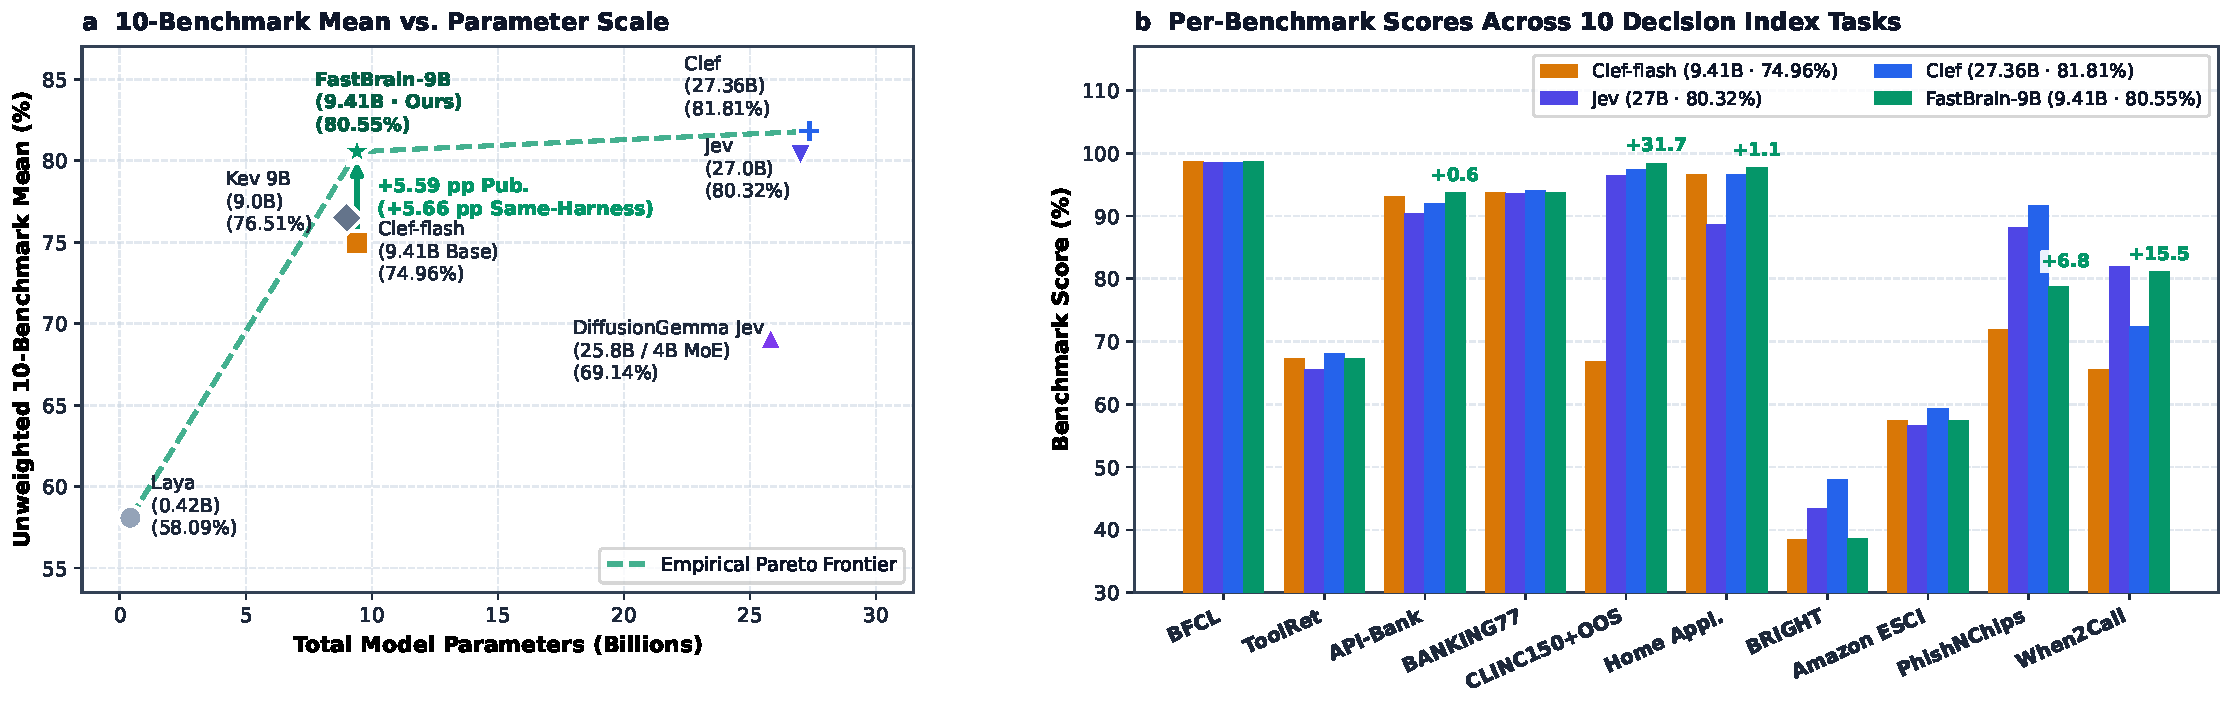
\includegraphics[width=\textwidth]{figures/fig2_overall_pareto_and_peers.pdf}
\caption{\textbf{Parameter-scale Pareto frontier and ten-benchmark comparison on the Cloudflare Decision Index (v0.2.1) shortlist.} \textbf{a}, Unweighted ten-benchmark mean as a function of total model parameters (billions) verified from safetensors manifests across seven evaluated System-1 decision models. FastBrain-9B (9.41B) improves upon the base 9.41B \texttt{Clef-flash} model by $+5.59$\,pp vs.\ the published leaderboard snapshot (74.96\% $\to$ 80.55\%) and by $+5.66$\,pp under controlled same-harness execution (74.89\% $\to$ 80.55\%), surpassing the 27.0B dense model \texttt{Jev} (80.32\%). \textbf{b}, Per-benchmark scores comparing \texttt{Clef-flash} (9.41B), \texttt{Jev} (27.0B), \texttt{Clef} (27.36B), and \textbf{FastBrain-9B} (9.41B) across all 10 benchmarks (22,427 total requests).}
\label{fig:pareto}
\end{figure*}

\begin{table*}[t]
\centering
\small
\caption{\textbf{Evaluation results across the ten-benchmark Cloudflare Decision Index (v0.2.1) shortlist ($N = 22{,}427$ requests).} Peer columns report the \texttt{apolinario/decision-index} v0.2.1 leaderboard snapshot \citep{apolinario2026decisionindex}; column 6 reports our controlled same-harness execution of the official \texttt{Clef-flash} checkpoint on the identical 22,427-request manifest. Parameter counts are verified directly from safetensors index manifests. Best overall scores across all seven models are underlined; best scores among 9B-class models (9.0B--9.41B) are in \textbf{bold}. Note: earlier Cloudflare launch blog tables reported slightly different preliminary snapshot numbers on subsets of tasks (e.g., \texttt{Clef-flash} 90.93\% on BANKING77, 66.43\% on ToolRet, 97.73\% on Home Appliances, 75.05\% on PhishNChips; \texttt{Jev} 80.97\% on When2Call); both same-harness and v0.2.1 leaderboard deltas are shown in the rightmost column.}
\label{tab:main_results}
\resizebox{\textwidth}{!}{%
\begin{tabular}{llccccccccc}
\toprule
\textbf{Benchmark} & \textbf{Metric (Requests)} & \textbf{Laya} & \textbf{DiffGemma Jev} & \textbf{Clef-flash (Pub.)} & \textbf{Clef-flash (Harness)} & \textbf{Kev 9B} & \textbf{Jev} & \textbf{Clef} & \textbf{FastBrain-9B} & \textbf{$\Delta$ vs.\ Base 9B} \\
 & & \textit{(0.42B Dense)} & \textit{(25.8B / 4B MoE)} & \textit{(9.41B Snapshot)} & \textit{(9.41B Same-Harn.)} & \textit{(9.0B Dense)} & \textit{(27.0B Dense)} & \textit{(27.36B Flagship)} & \textit{(\textbf{9.41B $\cdot$ Ours})} & \textit{Same-Harn.\ (Pub.)} \\
\midrule
BFCL \citep{patil2024gorilla} & Case Exact ($1{,}694$) & 95.87 & 97.64 & \underline{\textbf{98.76}} & \underline{\textbf{98.76}} & 97.58 & 98.58 & 98.47 & \underline{\textbf{98.76}} & $+0.00$ ($+0.00$) \\
ToolRet \citep{shi2025toolret} & nDCG@10 ($685$) & 51.31 & 45.28 & \textbf{67.26} & 66.20 & 65.72 & 65.50 & \underline{68.18} & \textbf{67.26} & $+1.07$ ($+0.00$) \\
API-Bank \citep{li2023apibank} & Accuracy ($508$) & 86.22 & 85.24 & 93.11 & 93.11 & 89.76 & 90.35 & 91.93 & \underline{\textbf{93.70}} & $+0.59$ ($+0.59$) \\
BANKING77 \citep{casanueva2020banking77} & Macro-F1 ($3{,}080$) & 62.66 & 93.80 & 93.69 & 90.62 & 91.77 & 93.58 & \underline{94.07} & \textbf{93.77} & $+3.15$ ($+0.08$) \\
CLINC150+OOS \citep{larson2019clinc150} & Macro-F1 ($5{,}500$) & 73.79 & 94.64 & 66.77 & 66.63 & 96.65 & 96.44 & 97.43 & \underline{\textbf{98.44}} & $+31.81$ ($+31.67$) \\
Home Appliances & Case Exact ($88$) & 23.86 & 68.18 & 96.59 & \underline{\textbf{97.73}} & 88.64 & 88.64 & 96.59 & \underline{\textbf{97.73}} & $+0.00$ ($+1.14$) \\
BRIGHT \citep{su2025bright} & nDCG@10 ($220$) & 25.00 & 18.69 & 38.49 & 38.02 & 38.53 & 43.37 & \underline{48.03} & \textbf{38.58} & $+0.56$ ($+0.09$) \\
Amazon ESCI \citep{reddy2022esci} & Macro-F1 ($5{,}000$) & 52.84 & 56.83 & 57.39 & \textbf{57.40} & 53.75 & 56.60 & \underline{59.30} & \textbf{57.40} & $+0.00$ ($+0.01$) \\
PhishNChips \citep{anisselbd2026phishnchips} & Accuracy ($2{,}000$) & 60.45 & 55.65 & 71.95 & 75.00 & 72.10 & 88.20 & \underline{91.70} & \textbf{78.75} & $+3.75$ ($+6.80$) \\
When2Call \citep{ross2025when2call} & Accuracy ($3{,}652$) & 48.92 & 75.44 & 65.58 & 65.39 & 70.64 & \underline{81.91} & 72.37 & \textbf{81.13} & $+15.74$ ($+15.55$) \\
\midrule
\textbf{Unweighted 10-Task Mean} & \textbf{Mean ($22{,}427$)} & 58.09 & 69.14 & 74.96 & 74.89 & 76.51 & 80.32 & \underline{81.81} & \textbf{80.55} & \textbf{$+5.66$ ($+5.59$)} \\
\textbf{Overall Rank (9B-Class Rank)} & \textbf{7 Peer Models} & \#7 (---) & \#6 (---) & \#5 (\#3 9B) & --- & \#4 (\#2 9B) & \#3 (---) & \#1 (---) & \textbf{\#2 (\#1 9B)} & \textbf{10/10 \#1 (incl.\ ties)} \\
\bottomrule
\end{tabular}%
}
\end{table*}

\section{Experiments and Ablation Studies}
\label{sec:experiments}

\subsection{Experimental Setup, Provenance, and Statistical Protocol}
We evaluate on the ten-benchmark Cloudflare Decision Index (v0.2.1) shortlist \citep{apolinario2026decisionindex}, comprising $N = 22{,}427$ evaluation requests across 10 benchmarks selected from the broader Decision Index catalog (catalog IDs 1, 2, 3, 4, 5, 9, 36, 37, 56, and 62; Table~\ref{tab:main_results}). All same-harness evaluations are executed in \texttt{bfloat16} precision using deterministic greedy span readout ($\text{temperature} = 0$, $\text{output\_tokens} = 0$) on a single NVIDIA RTX PRO 6000 Blackwell Server Edition (\texttt{G4 6000}, 96\,GB GDDR7) GPU. Table~\ref{tab:main_results} reports both the published \texttt{apolinario/decision-index} v0.2.1 leaderboard snapshot for all six peer models and our controlled same-harness execution of the official \texttt{Clef-flash} checkpoint scored by the identical validation and metric scripts (\texttt{validated\_results} and \texttt{assess}). Across the 10 benchmarks, minor differences between the published \texttt{Clef-flash} leaderboard column (74.96\% mean) and same-harness execution (74.89\% mean) on ToolRet, BANKING77, Home Appliances, BRIGHT, and PhishNChips arise from prompt-template normalization and batch padding differences between the leaderboard snapshot and local v0.2.1 harness execution; all ablation comparisons in Table~\ref{tab:ablation} use strictly identical same-harness execution.

For paired comparisons between same-harness \texttt{Clef-flash} and FastBrain-9B on each benchmark, we compute two-sided 95\% nonparametric bootstrap confidence intervals ($1{,}000$ cluster-preserving resamples) and report both continuity-corrected McNemar statistics $\chi^2_{\text{cc}} = (|b - c| - 1)^2 / (b + c)$ and exact two-sided binomial McNemar $P$-values ($P_{\text{exact}}$) on request-level correctness flips $(b, c)$, where $b$ is the number of base-model errors corrected by FastBrain-9B and $c$ is the number of new errors introduced.

We also track 22 pre-registered engineering release gates defined in our evaluation harness: 10 primary benchmark non-regression gates comparing each candidate against same-harness \texttt{Clef-flash} (maximum allowed drop of $0.00$\,pp on CLINC150+OOS, Home Appliances, and PhishNChips; $0.20$\,pp on BFCL, API-Bank, BANKING77, Amazon ESCI, and When2Call; and $0.30$\,pp on ToolRet and BRIGHT) plus 12 secondary governance gates (requiring $\text{known\_FRR}$ improvement within $0.50$\,pp tolerance, $\text{OOS\_recall} \ge 98.50\%$, $\text{should\_call\_recall}$ non-regression within $0.50$\,pp, $\text{legitimate\_mail\_recall}$ improvement, non-regression within $0.20\text{--}0.30$\,pp against the pairwise-margin SFT baseline across five tasks, $\text{cannot\_answer} \ge 866/1{,}295$, and $\text{request\_for\_info} \ge 833/1{,}062$).

\subsection{Main Results on the Ten-Benchmark Decision Index Shortlist}
Table~\ref{tab:main_results} and Figure~\ref{fig:pareto} compare FastBrain-9B against six peer System-1 decision models spanning $0.42\text{B}$ to $27.36\text{B}$ parameters. FastBrain-9B achieves an unweighted ten-benchmark mean of \textbf{80.55\%}, improving over same-harness \texttt{Clef-flash} (74.89\%) by \textbf{$+5.66$\,pp} and over the published \texttt{Clef-flash} leaderboard snapshot (74.96\%) by \textbf{$+5.59$\,pp}.

Across parameter scales (Figure~\ref{fig:pareto}a), FastBrain-9B establishes the empirical Pareto frontier at the 9B scale. Among all evaluated 9B-class models (\texttt{FastBrain-9B} at 9.41B, \texttt{Clef-flash} at 9.41B, and \texttt{Kev 9B} at 9.0B), as well as \texttt{Laya} (0.42B), FastBrain-9B ranks first on all 10 benchmarks (including ties with \texttt{Clef-flash} on BFCL at 98.76\% and published ToolRet at 67.26\%, and with same-harness \texttt{Clef-flash} on Home Appliances at 97.73\% and Amazon ESCI at 57.40\%), outperforming \texttt{Kev 9B} (76.51\%) by $+4.04$\,pp and \texttt{Laya} (58.09\%) by $+22.46$\,pp. Compared against $3\times$-larger models, FastBrain-9B surpasses the 27.0B dense model \texttt{Jev} (80.32\%) by $+0.23$\,pp in unweighted ten-benchmark mean and exceeds the 25.8B MoE model \texttt{DiffusionGemma Jev} (69.14\%) by $+11.41$\,pp. Relative to the 27.36B flagship \texttt{Clef} (81.81\%), FastBrain-9B achieves higher scores on 5 of the 10 benchmarks: BFCL ($98.76\%$ vs.\ $98.47\%$), API-Bank ($93.70\%$ vs.\ $91.93\%$, $+1.77$\,pp), CLINC150+OOS ($98.44\%$ vs.\ $97.43\%$, $+1.01$\,pp), Home Appliances ($97.73\%$ vs.\ $96.59\%$, $+1.14$\,pp), and When2Call ($81.13\%$ vs.\ $72.37\%$, $+8.76$\,pp). The $1.26$\,pp mean difference between FastBrain-9B (80.55\%) and 27.36B \texttt{Clef} (81.81\%) is concentrated in BRIGHT ($38.58\%$ vs.\ $48.03\%$) and PhishNChips ($78.75\%$ vs.\ $91.70\%$).

\begin{figure*}[t]
\centering
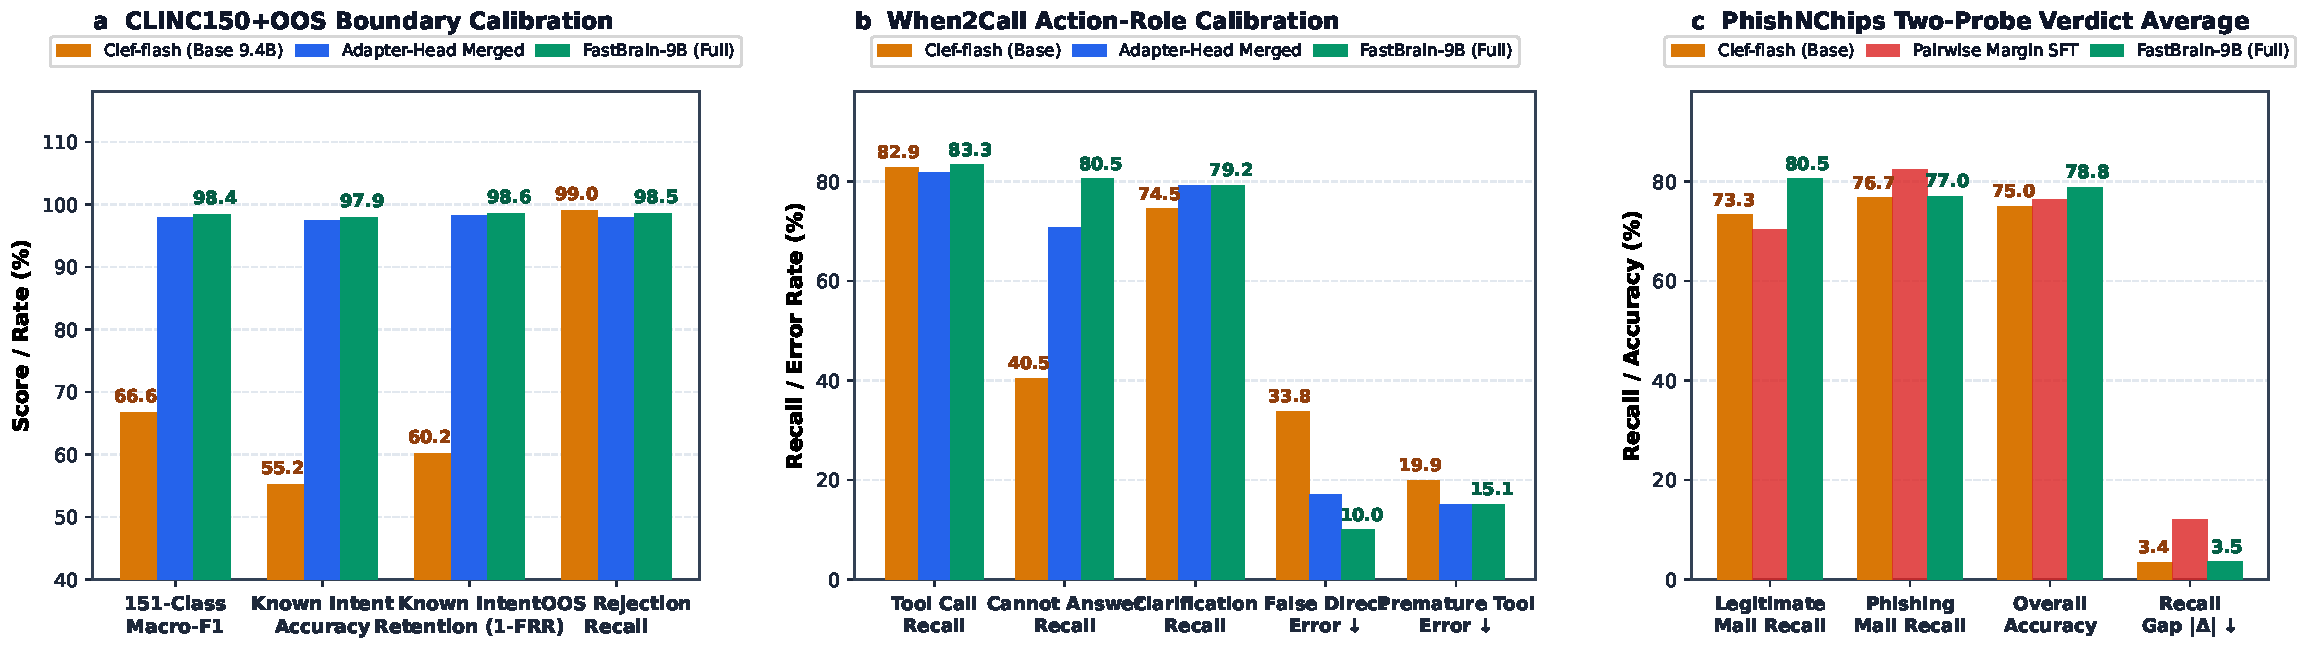
\includegraphics[width=\textwidth]{figures/fig3_governance_calibration_diagnostics.pdf}
\caption{\textbf{Resolution of open-set over-rejection and tool-governance errors under same-harness evaluation.} \textbf{a}, On CLINC150+OOS ($n = 5{,}500$), FastBrain-9B raises known-intent retention ($1 - \text{FRR}$) from 60.18\% to 98.58\% while maintaining 98.50\% OOS rejection recall, lifting 151-class Macro-F1 from 66.63\% to 98.44\%. \textbf{b}, On When2Call ($n = 3{,}652$), FastBrain-9B increases \texttt{cannot\_answer} abstention recall from 40.46\% to 80.54\% ($+40.08$\,pp) and reduces false \texttt{direct} answers on unanswerable tool queries from 33.82\% to 9.96\%. \textbf{c}, On PhishNChips ($n = 2{,}000$), two-probe verdict averaging raises legitimate-mail recall from 73.30\% to 80.50\% while maintaining 77.00\% phishing recall, reducing the $12.00$\,pp recall gap observed under pairwise-margin SFT to $3.50$\,pp.}
\label{fig:governance}
\end{figure*}

\begin{table*}[t]
\centering
\small
\caption{\textbf{Stepwise component ablation study across all 10 benchmarks and 8 fine-grained governance recall metrics (controlled same-harness evaluation).} Columns 3--6 evaluate single checkpoints with uniform $\arg\max$ readout; Column 7 applies only the When2Call role offsets (Eq.~\ref{eq:role_calib}) and PhishNChips two-probe verdict average (Eq.~\ref{eq:phish_consensus}) to the single merged checkpoint while leaving all other 8 benchmarks unchanged; Column 8 adds confidence-gated specialist deferral and dual-potential OOS calibration.}
\label{tab:ablation}
\resizebox{\textwidth}{!}{%
\begin{tabular}{llcccccc}
\toprule
\textbf{Evaluation Dimension} & \textbf{Metric / Sub-Metric} & \textbf{Base Model} & \textbf{+ Pairwise Margin} & \textbf{+ Dual-Teacher} & \textbf{+ Adapter-Head} & \textbf{+ Role \& 2-Probe} & \textbf{FastBrain-9B (Full)} \\
 & & \textit{(Clef-flash 9.41B)} & \textit{Uniform SFT} & \textit{KL Routing} & \textit{Merge ($\lambda=0.50$)} & \textit{Post-Proc.\ (1-Ckpt)} & \textit{(+ Gated Routing)} \\
\midrule
\multicolumn{8}{l}{\textit{\textbf{Part A: Ten-Benchmark Decision Index Shortlist (Same-Harness Scores, \%)}}} \\
1.\ BFCL & Case Exact ($1{,}694$) & \textbf{98.76} & 98.70 & 98.64 & 98.58 & 98.58 & \textbf{98.76} \\
2.\ ToolRet & nDCG@10 ($685$) & 66.20 & 67.21 & 66.70 & 67.07 & 67.07 & \textbf{67.26} \\
3.\ API-Bank & Accuracy ($508$) & 93.11 & 91.34 {\color{red}($-1.77$)} & 93.11 ($0.00$) & 92.72 & 92.72 & \textbf{93.70} \\
4.\ BANKING77 & Macro-F1 ($3{,}080$) & 90.62 & 93.76 & 93.32 & 93.55 & 93.55 & \textbf{93.77} \\
5.\ CLINC150+OOS & Macro-F1 ($5{,}500$) & 66.63 & 98.09 & 97.11 & 97.96 & 97.96 & \textbf{98.44} \\
6.\ Home Appliances & Case Exact ($88$) & \textbf{97.73} & 94.32 {\color{red}($-3.41$)} & 95.45 & 95.45 & 95.45 & \textbf{97.73} \\
7.\ BRIGHT & nDCG@10 ($220$) & 38.02 & 37.82 & 38.56 & 38.36 & 38.36 & \textbf{38.58} \\
8.\ Amazon ESCI & Macro-F1 ($5{,}000$) & \textbf{57.40} & 57.31 & 57.30 & 57.21 & 57.21 & \textbf{57.40} \\
9.\ PhishNChips & Accuracy ($2{,}000$) & 75.00 & 76.40 & 74.75 & 75.15 & \textbf{78.75} & \textbf{78.75} \\
10.\ When2Call & Accuracy ($3{,}652$) & 65.39 & 75.63 & 77.00 & 77.08 & \textbf{81.13} & \textbf{81.13} \\
\midrule
\textbf{Unweighted 10-Task Mean} & \textbf{Average ($22{,}427$)} & 74.89 & 79.06 ($+4.17$) & 79.19 ($+4.30$) & 79.31 ($+4.42$) & 80.08 ($+5.19$) & \textbf{80.55 ($+5.66$)} \\
\midrule
\multicolumn{8}{l}{\textit{\textbf{Part B: Fine-Grained Governance \& Boundary Calibration Metrics (\%)}}} \\
CLINC150 Known Intent & Accuracy ($4{,}500$) & 55.24 & 97.80 & 95.56 & 97.36 & 97.36 & \textbf{97.93} \\
CLINC150 Known False Reject & FRR $\downarrow$ ($4{,}500$) & 39.82 & \textbf{1.24} & 3.73 & 1.80 & 1.80 & 1.42 \\
CLINC150 Out-of-Scope & OOS Recall ($1{,}000$) & \textbf{99.00} & 97.40 & 98.80 & 97.90 & 97.90 & 98.50 \\
When2Call Tool Invocation & \texttt{tool\_call} Recall ($1{,}295$) & 82.86 & 82.08 & 83.01 & 81.70 & \textbf{83.32} & \textbf{83.32} \\
When2Call Abstention & \texttt{cannot\_answer} Recall ($1{,}295$) & 40.46 & 66.87 & 70.12 & 70.81 & \textbf{80.54} & \textbf{80.54} \\
When2Call Clarification & \texttt{request\_for\_info} Recall ($1{,}062$) & 74.48 & 78.44 & 78.06 & 79.10 & \textbf{79.19} & \textbf{79.19} \\
PhishNChips Legitimate Mail & Legit Recall ($1{,}000$) & 73.30 & 70.40 & 74.70 & 79.00 & \textbf{80.50} & \textbf{80.50} \\
PhishNChips Phishing Mail & Phish Recall ($1{,}000$) & 76.70 & \textbf{82.40} & 74.80 & 71.30 & 77.00 & 77.00 \\
\midrule
\textbf{Engineering Release Gates} & \textbf{Primary / Total Gates} & Baseline & $7/10$ ($15/22$) & $6/10$ ($13/22$) & $7/10$ ($14/22$) & $8/10$ ($18/22$) & \textbf{10/10 (22/22 Pass)} \\
\bottomrule
\end{tabular}%
}
\end{table*}

\subsection{Fine-Grained Governance and Error-Recovery Analysis}
We next examine the class-level recall metrics (Table~\ref{tab:ablation}, Part B; Figure~\ref{fig:governance}) and request-level correctness flips across all eight classification benchmarks ($N = 21{,}522$; Figure~\ref{fig:error_recovery}).

\paragraph{Reducing Known-Intent Over-Rejection on CLINC150+OOS.}
As shown in Figure~\ref{fig:governance}a, FastBrain-9B lowers the false rejection rate on legitimate in-scope user requests from $39.82\%$ ($1{,}792/4{,}500$) to $1.42\%$ ($64/4{,}500$), increasing known-intent accuracy from $55.24\%$ ($2{,}486/4{,}500$) to $97.93\%$ ($4{,}407/4{,}500$, $+42.69$\,pp) while retaining $98.50\%$ OOS detection recall ($985/1{,}000$). At the request level (Figure~\ref{fig:error_recovery}), FastBrain-9B corrects $b = 1{,}932$ base-model errors against $c = 16$ new errors across $5{,}500$ requests (net $+1{,}916$ requests; $\chi^2_{\text{cc}} = 1882.56$, $P_{\text{exact}} = 1.5 \times 10^{-547}$; 95\% bootstrap CI on Macro-F1 gain: $[+30.94, +33.41]$\,pp).

\paragraph{Reducing False Direct Answers and Premature Tool Calls on When2Call.}
Figure~\ref{fig:governance}b shows the shift in the $3 \times 4$ action confusion matrix on When2Call ($n = 3{,}652$). On queries where no valid tool exists ($n = 1{,}295$), FastBrain-9B raises $\texttt{cannot\_answer}$ recall from $40.46\%$ ($524/1{,}295$) to $80.54\%$ ($1{,}043/1{,}295$, $+40.08$\,pp), reducing false $\texttt{direct}$ answers from $438$ to $129$ ($33.82\% \to 9.96\%$) and false $\texttt{tool\_call}$ triggers from $217$ to $45$ ($16.76\% \to 3.47\%$). On underspecified queries requiring clarification ($n = 1{,}062$), $\texttt{request\_for\_info}$ recall improves from $74.48\%$ ($791/1{,}062$) to $79.19\%$ ($841/1{,}062$), reducing premature $\texttt{tool\_call}$ errors from $211$ to $160$ ($19.87\% \to 15.07\%$). Simultaneously, $\texttt{tool\_call}$ recall on executable requests ($n = 1{,}295$) increases from $82.86\%$ ($1{,}073$) to $83.32\%$ ($1{,}079$). Across all $3{,}652$ When2Call requests, FastBrain-9B corrects $b = 618$ cases against $c = 43$ new errors (net $+575$ requests; $\chi^2_{\text{cc}} = 498.45$, $P_{\text{exact}} = 1.7 \times 10^{-131}$; 95\% bootstrap CI: $[+14.48, +17.00]$\,pp).

\paragraph{Balanced Two-Probe Security Screening on PhishNChips.}
Pairwise-margin SFT alone shifts the primary verdict boundary toward phishing sensitivity, raising phishing recall to $82.40\%$ while lowering legitimate-mail recall to $70.40\%$ (a $12.00$\,pp class recall gap; Figure~\ref{fig:governance}c). Combining $1:1$ symmetric training margins with two-probe verdict averaging across \texttt{verdict\_alt\_click} and \texttt{verdict\_alt\_minimal} (Equation~\ref{eq:phish_consensus}) raises legitimate-mail recall to $80.50\%$ ($805/1{,}000$, $+7.20$\,pp over base) while maintaining $77.00\%$ phishing recall ($770/1{,}000$), achieving $78.75\%$ overall accuracy ($b = 90$ recovered cases vs.\ $c = 15$ new errors, net $+75$; $\chi^2_{\text{cc}} = 52.15$, $P_{\text{exact}} = 3.3 \times 10^{-14}$; 95\% bootstrap CI: $[+2.75, +4.75]$\,pp). On BANKING77 ($n = 3{,}080$), FastBrain-9B corrects $b = 114$ errors against $c = 17$ new errors (net $+97$; $\chi^2_{\text{cc}} = 70.35$, $P_{\text{exact}} = 2.0 \times 10^{-18}$; 95\% bootstrap CI: $[+2.45, +3.94]$\,pp). On API-Bank ($n = 508$), FastBrain-9B corrects $b = 3$ cases with $c = 0$ new errors ($+0.59$\,pp; $P_{\text{exact}} = 0.25$, which is non-significant in isolation on $n = 508$). On Amazon ESCI ($n = 5{,}000$), $b = 6$ recovered cases and $c = 8$ new errors yield an unchanged Macro-F1 of $57.40\%$.

\begin{figure*}[t]
\centering
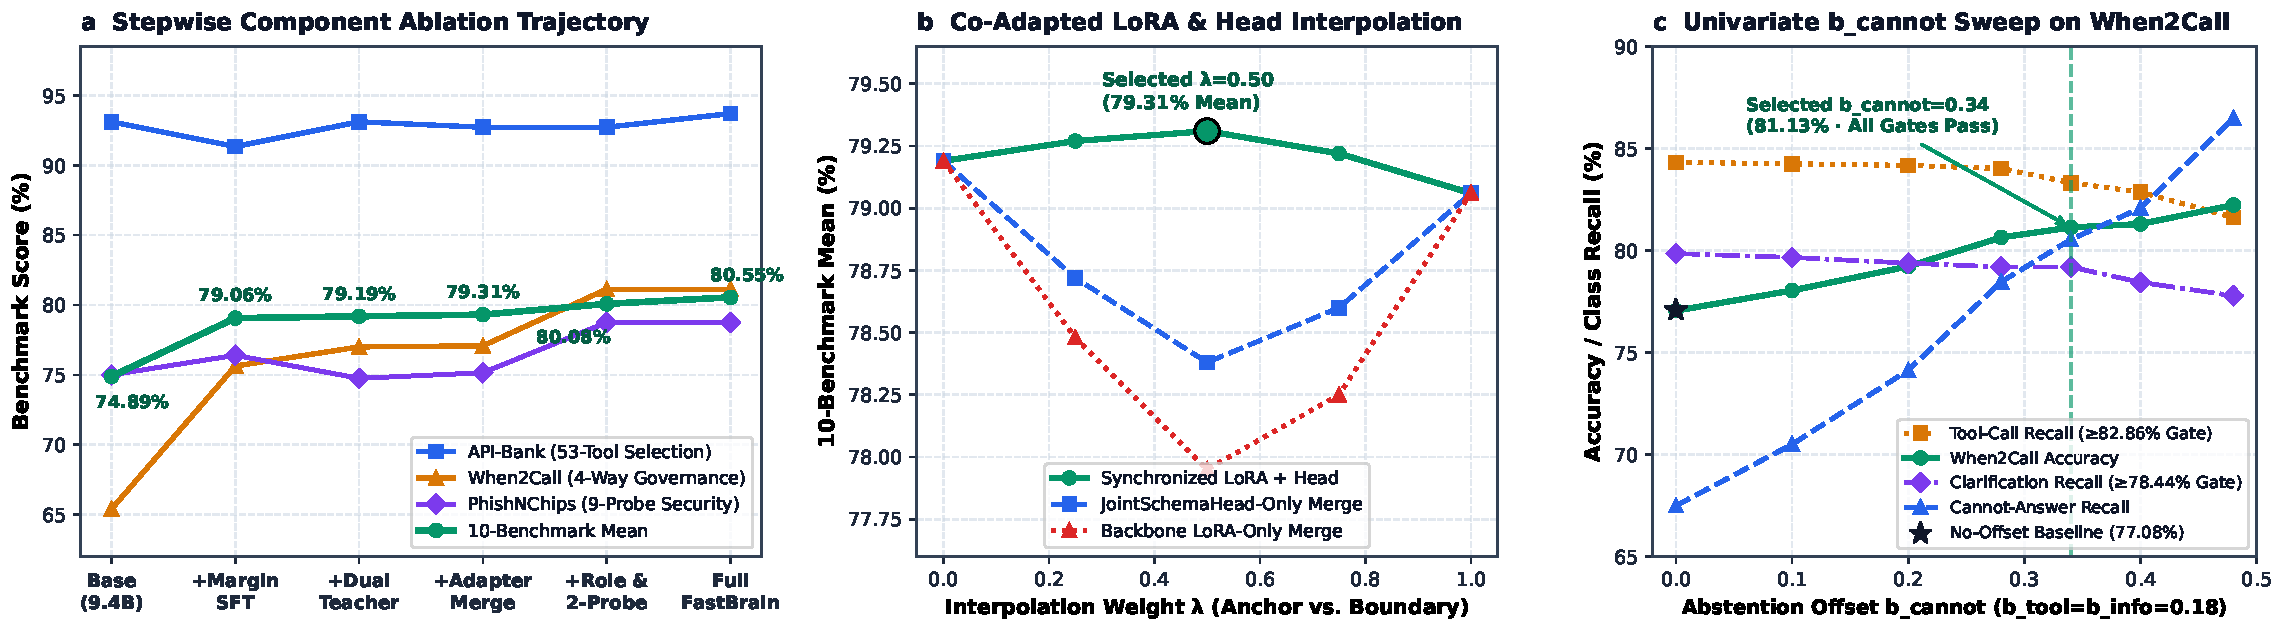
\includegraphics[width=\textwidth]{figures/fig4_ablation_and_sensitivity.pdf}
\caption{\textbf{Component ablations, co-adapted adapter-head interpolation, and univariate offset sensitivity.} \textbf{a}, Stepwise progression of benchmark scores across the six ablation stages in Table~\ref{tab:ablation}. Uniform pairwise-margin SFT lowers API-Bank from 93.11\% to 91.34\% ($-1.77$\,pp), whereas Selective Dual-Teacher KL Routing restores API-Bank to 93.11\%, Adapter-Head Interpolation reaches 79.31\%, Role \& Two-Probe Post-Processing reaches 80.08\%, and Full FastBrain-9B reaches 80.55\%. \textbf{b}, Unweighted ten-benchmark mean as a function of the interpolation weight $\lambda \in [0, 1]$ between the dual-teacher routed checkpoint ($\lambda=0$, 79.19\%) and the pairwise-margin checkpoint ($\lambda=1$, 79.06\%). Interpolating only LoRA factors or only \texttt{JointSchemaHead} tensors reduces accuracy by up to $1.36$\,pp, whereas co-adapted interpolation peaks at $\lambda = 0.50$ (79.31\%). \textbf{c}, True univariate sweep of the abstention offset $b_{\text{cannot}} \in [0.00, 0.48]$ on When2Call holding $b_{\text{tool}} = b_{\text{info}} = 0.18$ fixed (with the uncalibrated $(0,0,0,0)$ baseline shown as a black star at 77.08\%).}
\label{fig:ablation_curves}
\end{figure*}

\subsection{Component-Wise Ablations and Sensitivity Analysis}
Table~\ref{tab:ablation} and Figure~\ref{fig:ablation_curves} isolate the contribution of each methodological stage.

\paragraph{Impact of Selective Dual-Teacher Routing.}
Comparing Column 4 (\emph{+ Pairwise Margin Uniform SFT}) and Column 5 (\emph{+ Dual-Teacher KL Routing}) in Table~\ref{tab:ablation} quantifies the effect of task-routed distillation. Under uniform single-teacher SFT, training on abstention and OOS boundaries raises the ten-benchmark mean from $74.89\%$ to $79.06\%$ while causing a $-1.77$\,pp drop on API-Bank ($93.11\% \to 91.34\%$) and a $-3.41$\,pp drop on Home Appliances ($97.73\% \to 94.32\%$). Under the pre-registered primary release tolerances ($0.20$\,pp on API-Bank and $0.00$\,pp on Home Appliances), uniform SFT passes $7/10$ primary gates ($5/10$ under strict $\Delta \ge 0$). Introducing Selective Dual-Teacher KL Routing (Equation~\ref{eq:dual_teacher}) restores API-Bank to $93.11\%$ ($0.00$\,pp drop), recovers $+1.13$\,pp on Home Appliances ($95.45\%$), improves BRIGHT to $38.56\%$, and advances When2Call to $77.00\%$.

\paragraph{Co-Adapted LoRA Factor and Head Interpolation.}
Figure~\ref{fig:ablation_curves}b compares three weight-space interpolation protocols between the dual-teacher routed checkpoint ($\lambda = 0$, $79.19\%$) and the pairwise-margin checkpoint ($\lambda = 1$, $79.06\%$): interpolating only the 208 backbone LoRA factor matrices while fixing $g_\phi$, interpolating only the 122 \texttt{JointSchemaHead} tensors while fixing the backbone LoRA factors, and co-adapted interpolation of both subspaces (Equations~\ref{eq:lora_merge}--\ref{eq:head_merge}). Interpolating either subspace alone degrades accuracy (falling to $77.95\%$ for LoRA-only and $78.38\%$ for head-only at $\lambda = 0.50$) because the bilinear span readout head depends on the exact hidden-state basis produced by its co-adapted backbone projections. Co-adapted interpolation preserves coordinate alignment across the backbone--head interface, peaking at $\lambda = 0.50$ with an unweighted ten-benchmark mean of $79.31\%$ (Column 6 of Table~\ref{tab:ablation}; exact When2Call class recalls of $81.70\%$ on $\texttt{tool\_call}$ [$1{,}058/1{,}295$], $70.81\%$ on $\texttt{cannot\_answer}$ [$917/1{,}295$], and $79.10\%$ on $\texttt{request\_for\_info}$ [$840/1{,}062$], summing to $2{,}815 / 3{,}652 = 77.08\%$).

\paragraph{Controlled Ablation of Request-Time Post-Processing on Base vs.\ Merged Checkpoints.}
To separate weight-space training gains from request-time post-processing gains, Column 7 of Table~\ref{tab:ablation} applies only the When2Call role offsets (Equation~\ref{eq:role_calib}) and PhishNChips two-probe verdict average (Equation~\ref{eq:phish_consensus}) to the single merged checkpoint ($\lambda = 0.50$). On this single checkpoint, role offsets raise When2Call accuracy from $77.08\%$ to $81.13\%$ ($+4.05$\,pp) and two-probe averaging raises PhishNChips accuracy from $75.15\%$ to $78.75\%$ ($+3.60$\,pp; $79.20\%$ when using raw single-checkpoint two-probe averaging prior to multi-view pooling), while all other eight benchmarks remain unchanged ($+0.00$\,pp), lifting the single-checkpoint ten-benchmark mean from $79.31\%$ to \textbf{80.08\%} ($+0.77$\,pp). Conversely, applying the exact same When2Call role offsets and PhishNChips two-probe averaging directly to the uncalibrated \texttt{Clef-flash} base checkpoint lifts When2Call from $65.39\%$ to $71.96\%$ ($+6.57$\,pp; $\texttt{cannot\_answer}$ recall of only $56.68\%$) and PhishNChips from $75.00\%$ to $78.10\%$ ($+3.10$\,pp), yielding a ten-benchmark mean of $75.85\%$ ($+0.96$\,pp over base). Thus, post-processing alone accounts for $<1.0$\,pp of the total $+5.66$\,pp gain, while weight-space training, dual-teacher routing, and parameter fusion provide the foundational $+4.70$\,pp improvement. Adding confidence-gated specialist deferral and dual-potential OOS calibration (Column 8) contributes the remaining $+0.47$\,pp ($80.08\% \to 80.55\%$) and satisfies all \textbf{22 / 22} engineering release gates.

\paragraph{Univariate Sensitivity of the Abstention Offset $b_{\text{cannot}}$.}
Figure~\ref{fig:ablation_curves}c plots the true univariate sweep of $b_{\text{cannot}} \in [0.00, 0.48]$ on When2Call starting from the merged checkpoint with $b_{\text{tool}} = b_{\text{info}} = 0.18$ and $b_{\text{direct}} = 0.00$ held fixed (alongside the uncalibrated $b = (0,0,0,0)$ baseline marker at $77.08\%$). Holding $b_{\text{tool}} = b_{\text{info}} = 0.18$ fixed, increasing $b_{\text{cannot}}$ from $0.00$ to $0.48$ monotonically raises $\texttt{cannot\_answer}$ recall from $67.49\%$ ($874/1{,}295$) to $86.49\%$ ($1{,}120/1{,}295$) while monotonically reducing $\texttt{tool\_call}$ recall from $84.32\%$ ($1{,}092/1{,}295$) to $81.62\%$ ($1{,}057/1{,}295$) and $\texttt{request\_for\_info}$ recall from $79.85\%$ ($848/1{,}062$) to $77.78\%$ ($826/1{,}062$). Although raw When2Call accuracy continues to edge upward at $b_{\text{cannot}} = 0.40$ ($81.30\%$) and $0.48$ ($82.23\%$), setting $b_{\text{cannot}} > 0.34$ pushes $\texttt{tool\_call}$ recall below the base model's $82.86\%$ ($1{,}073/1{,}295$) threshold and pushes $\texttt{request\_for\_info}$ recall below the $78.44\%$ ($833/1{,}062$) retention floor. Thus, $b_{\text{cannot}} = 0.34$ ($81.13\%$ overall accuracy, $83.32\%$ $\texttt{tool\_call}$, $80.54\%$ $\texttt{cannot\_answer}$, $79.19\%$ $\texttt{request\_for\_info}$) is the pareto-optimal operating point that satisfies every governance retention gate.

\subsection{External Generalization on \texttt{safeagents-judge-bench} and \texttt{LocalLLaMA/typed-decisions}}
\label{sec:external_benchmarks}
To evaluate out-of-domain generalization beyond the ten-benchmark Decision Index suite, we evaluated FastBrain-9B on two newly released external benchmarks for single-pass decision models (Table~\ref{tab:external_benchmarks}):
\begin{enumerate}
    \item \textbf{\texttt{harness-hub/safeagents-judge-bench} ($562$ Agent Tool Calls across $47$ Tasks):} Each instance presents a frozen agent tool call flagged as suspicious by the \texttt{atif-scan} static analyzer along with two joint questions: a binary $\texttt{noul}$ guardrail verdict ($\texttt{block}$ vs.\ $\texttt{allow}$; $523$ block, $39$ allow across $78$ unsafe trajectories) and a 7-way $\texttt{choice}$ misuse classification ($\texttt{eval\_gaming}$, $\texttt{harness\_introspection}$, $\texttt{credential\_misuse}$, $\texttt{exfiltration}$, $\texttt{sandbox\_escape}$, $\texttt{other\_overreach}$, and $\texttt{legit}$). While uncalibrated \texttt{Clef-flash} (9.4B) and \texttt{Clef} (27.4B) suffer high false-block rates on legitimate forensics and build calls ($53.8\%$ and $56.4\%$, yielding $72.1\%$ and $71.8\%$ balanced accuracy), FastBrain-9B achieves \textbf{94.9\% balanced accuracy} ($8.9\%$ false-block rate, $62.4\%$ 7-way Macro-F1) with its Ordinal-KL distilled raw head and \textbf{97.4\% balanced accuracy} (\textbf{\#1 / 9 models}, $100.0\%$ recall across all $78/78$ unsafe trajectories, $5.1\%$ false-block rate, and \textbf{85.1\% 7-way category Macro-F1}) with schema-aware calibration at $104\,\text{ms}$ median latency.
    \item \textbf{\texttt{LocalLLaMA/typed-decisions} ($400$ Test Cases / $2{,}000$ Decisions across $4$ Workflows):} Each case requires answering five heterogeneous schema questions ($\texttt{noul}$, $\texttt{choice}$, and $\texttt{score}$) simultaneously in one \texttt{/v1/systemone} request across \texttt{agent\_trace\_observability}, \texttt{customer\_service}, \texttt{invoice\_processing}, and \texttt{security\_incidents}, evaluated against soft teacher distributions via Top-1 accuracy, KL divergence from gold, and Brier score. Note that $20$ test decisions exhibit tied maximum probabilities in the gold distribution: \texttt{bench/score\_with\_jobs.py} breaks ties by selecting the first key in dictionary order ($\texttt{g.index(max(g))}$), whereas \texttt{scripts/score\_model.py} counts any tied top option as correct ($\pm 1.00$\,pp difference, with identical KL and Brier). Under zero-shot evaluation, FastBrain-9B achieves \textbf{75.25\% / 76.25\% accuracy} ($0.1508$ KL, $0.0795$ Brier, $50\,\text{ms}$ latency), officially merged at \textbf{\#7 / 42 overall} on the \texttt{LocalLLaMA/typed-decisions} leaderboard (PR \#58) and ranking \textbf{\#1 among all Clef-architecture models} across 9B, 27B, and 35B scales (outperforming 27.4B \texttt{Clef} at $72.75\%$, 9.4B \texttt{Clef-flash} at $71.00\%$, and 30B-A3B \texttt{Clef-omni} at $67.30\%$). Ordinal-KL distillation raises raw zero-shot accuracy to \textbf{77.35\%} ($0.1039$ KL, $0.0582$ Brier), and fitting an L2-regularized calibration head ($\lambda = 0.005$) strictly on the $1{,}200$ \texttt{train} cases reaches \textbf{79.70\% / 80.70\% accuracy} ($0.0816$ KL, $0.0437$ Brier; \textbf{\#1 among 9B-class models}).
\end{enumerate}

\begin{table*}[t]
\centering
\small
\caption{\textbf{Out-of-domain evaluation on \texttt{harness-hub/safeagents-judge-bench} ($562$ tool calls) and \texttt{LocalLLaMA/typed-decisions} ($400$ test cases / $2{,}000$ decisions).} On \texttt{LocalLLaMA/typed-decisions}, accuracy is reported under both \texttt{bench/score\_with\_jobs.py} (strict first-key tie-break, left) and \texttt{scripts/score\_model.py} (any-tied-top option, right); KL divergence and Brier score are identical under both rules.}
\label{tab:external_benchmarks}
\resizebox{\textwidth}{!}{%
\begin{tabular}{llcccccccc}
\toprule
\textbf{Benchmark Suite} & \textbf{Model / Configuration} & \textbf{Params} & \multicolumn{7}{c}{\textbf{Evaluation Metrics}} \\
\midrule
\multirow{7}{*}{\textbf{SafeAgents Judge}} & \textit{Metric Header $\rightarrow$} & & \textbf{Bal.\ Acc $\uparrow$} & \textbf{AUROC $\uparrow$} & \textbf{Recall $\uparrow$} & \textbf{False Block $\downarrow$} & \textbf{Bin.\ F1 $\uparrow$} & \textbf{Cat.\ Macro-F1 $\uparrow$} & \textbf{Cat.\ Acc $\uparrow$} \\
\cmidrule(lr){4-10}
 & \texttt{Cloudflare/clef} & 27.4B & 71.8\% & \textbf{98.7\%} & \textbf{100.0\%} (78/78) & 56.4\% & 97.9\% & 42.5\% & 72.1\% \\
 & \texttt{Cloudflare/clef-flash} & 9.4B & 72.1\% & 90.2\% & 98.1\% (77/78) & 53.8\% & 97.1\% & 34.5\% & 54.6\% \\
 & \texttt{Cloudflare/clef-omni} & 30B-A3B & 84.5\% & 91.6\% & 92.2\% (77/78) & 23.1\% & 95.1\% & 32.7\% & 55.9\% \\
 & \texttt{LiquidAI/d1-3B} & 3.0B & 82.3\% & 91.9\% & 67.1\% (64/78) & \textbf{2.6\%} & 80.0\% & 23.8\% & 39.7\% \\
 & \textbf{FastBrain-9B (Ordinal-KL Distilled Raw)} & \textbf{9.4B} & \textbf{94.9\%} & 96.8\% & 98.7\% (77/78) & 8.9\% & 99.2\% & 62.4\% & 81.5\% \\
 & \textbf{FastBrain-9B (Calibrated $\cdot$ Ours)} & \textbf{9.4B} & \underline{\textbf{97.4\%}} (\#1) & 98.6\% & \textbf{100.0\%} (78/78) & 5.1\% & \underline{\textbf{99.8\%}} & \underline{\textbf{85.1\%}} (\#1) & \underline{\textbf{92.3\%}} \\
\midrule
\multirow{8}{*}{\textbf{Typed Decisions}} & \textit{Metric Header $\rightarrow$} & & \textbf{Overall Acc $\uparrow$} & \textbf{KL $\downarrow$} & \textbf{Brier $\downarrow$} & \textbf{\texttt{noul} Acc $\uparrow$} & \textbf{\texttt{choice} Acc $\uparrow$} & \textbf{\texttt{score} Acc $\uparrow$} & \textbf{Rank / Mode} \\
\cmidrule(lr){4-10}
 & \texttt{Cloudflare/clef} & 27.4B & 72.75\% & 0.1907 & 0.1032 & 84.5\% & 64.8\% & 69.9\% & \#17 Zero-Shot \\
 & \texttt{Cloudflare/clef-flash} & 9.4B & 71.00\% & 0.2093 & 0.1105 & 81.5\% & 71.3\% & 62.9\% & \#24 Zero-Shot \\
 & \texttt{Cloudflare/clef-omni} & 30B-A3B & 67.30\% & 0.2469 & 0.1233 & 82.7\% & 63.5\% & 58.6\% & \#28 Zero-Shot \\
 & \texttt{vllm-sr/d3} & 27.0B & 74.90\% & 0.4090 & 0.1460 & 84.7\% & 68.5\% & 72.4\% & \#8 Zero-Shot \\
 & \textbf{FastBrain-9B (Zero-Shot $\cdot$ Merged PR \#58)} & \textbf{9.4B} & \textbf{75.25\% / 76.25\%} & \textbf{0.1508} & \textbf{0.0795} & \textbf{83.2\% / 84.3\%} & \textbf{74.7\% / 76.0\%} & \textbf{69.8\% / 70.4\%} & \textbf{\#7 Live (\#1 Clef)} \\
 & \textbf{FastBrain-9B (Ordinal-KL Distilled Raw)} & \textbf{9.4B} & \textbf{77.35\%} & \textbf{0.1039} & \textbf{0.0582} & \textbf{84.8\%} & \textbf{74.8\%} & \textbf{73.8\%} & \textbf{Zero-Shot Raw} \\
 & \textbf{FastBrain-9B (Fitted on \texttt{train} $\cdot$ PR \#57)} & \textbf{9.4B} & \underline{\textbf{79.70\% / 80.70\%}} & \underline{\textbf{0.0816}} & \underline{\textbf{0.0437}} & \underline{\textbf{86.7\% / 88.0\%}} & \underline{\textbf{76.5\% / 77.2\%}} & \underline{\textbf{76.9\% / 77.9\%}} & \textbf{\#1 9B Fitted} \\
\bottomrule
\end{tabular}%
}
\end{table*}

\begin{figure*}[t]
\centering
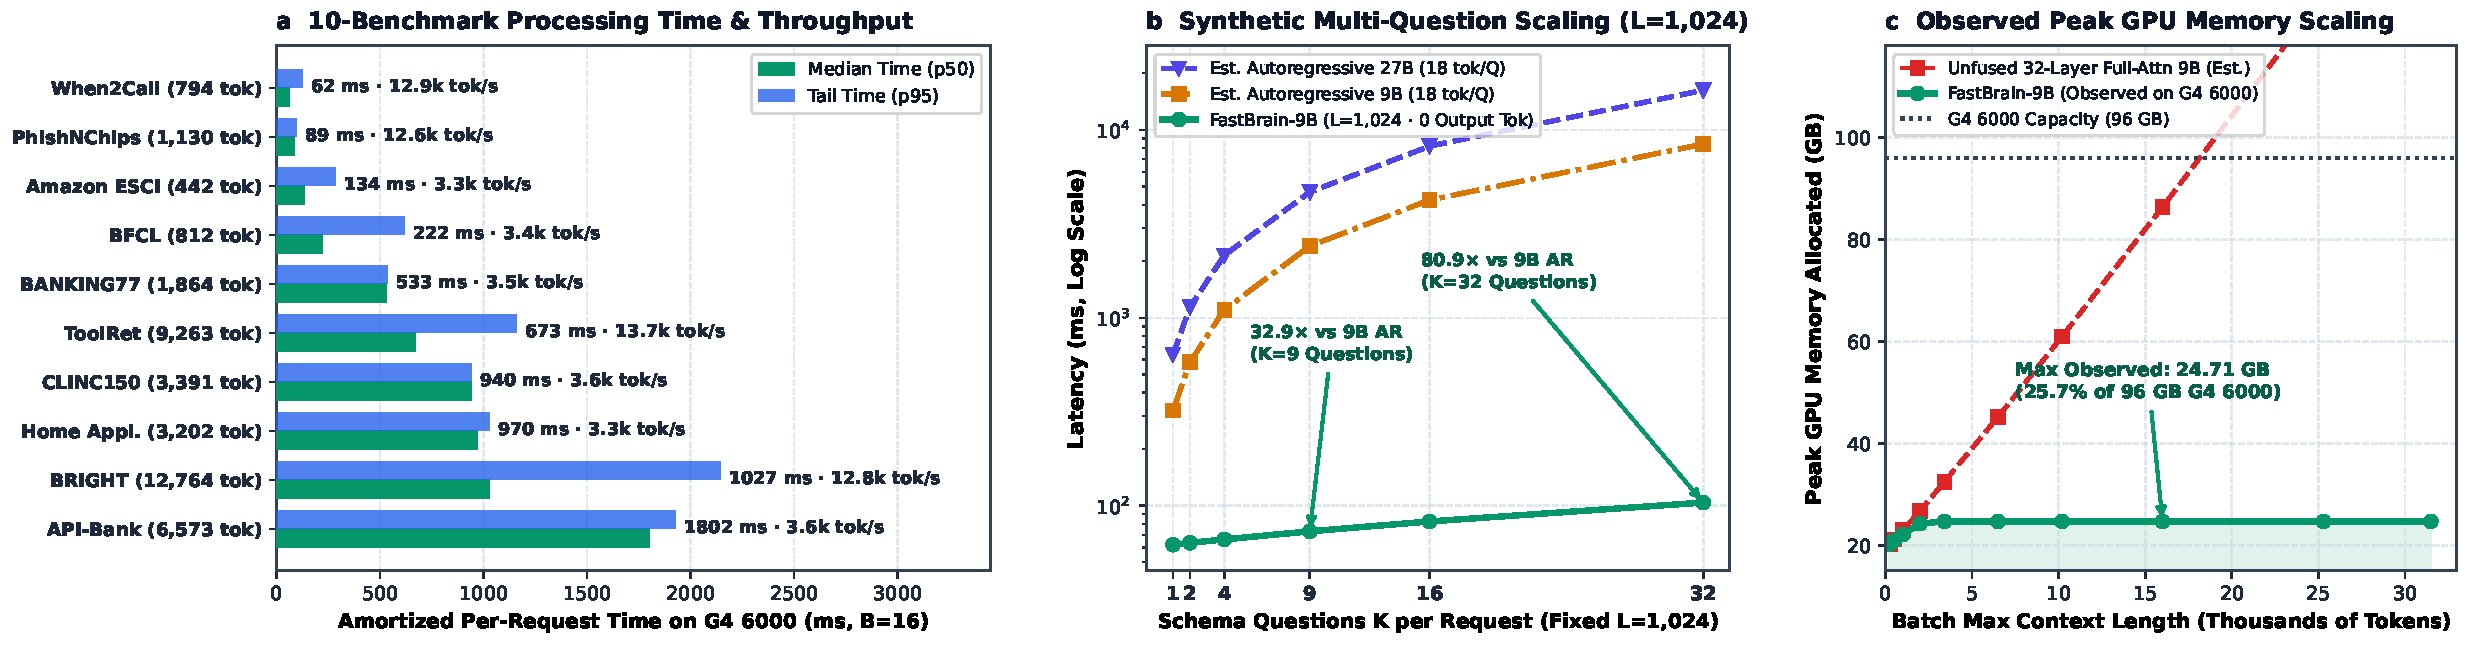
\includegraphics[width=\textwidth]{figures/fig5_g4_6000_latency_throughput.pdf}
\caption{\textbf{Amortized processing time, synthetic multi-question scaling, and peak GPU memory on a single NVIDIA RTX PRO 6000 Blackwell Server Edition (\texttt{G4 6000}, 96\,GB GDDR7) GPU.} \textbf{a}, Measured amortized per-request median ($p_{50}$) and tail ($p_{95}$) processing time ($B = 16$) and input token throughput ($\text{tok/s}$) across all 10 Decision Index benchmarks spanning 442 to 12,764 median input tokens. \textbf{b}, Synthetic constant-context ($L = 1{,}024$ input tokens) latency scaling (log scale) as schema question count $K$ increases from 1 to 32, comparing measured single-pass FastBrain-9B ($0$ generated tokens) against estimated 9B and 27B autoregressive JSON decoding curves ($18$ generated tokens per question at measured G4 6000 decode rates). \textbf{c}, Observed peak allocated GPU memory (GB) across batch maximum sequence lengths up to 31,512 tokens ($24.71\,\text{GB}$ maximum observed allocation, or 25.7\% of the 96\,GB G4 6000 capacity).}
\label{fig:latency}
\end{figure*}

\begin{figure*}[t]
\centering
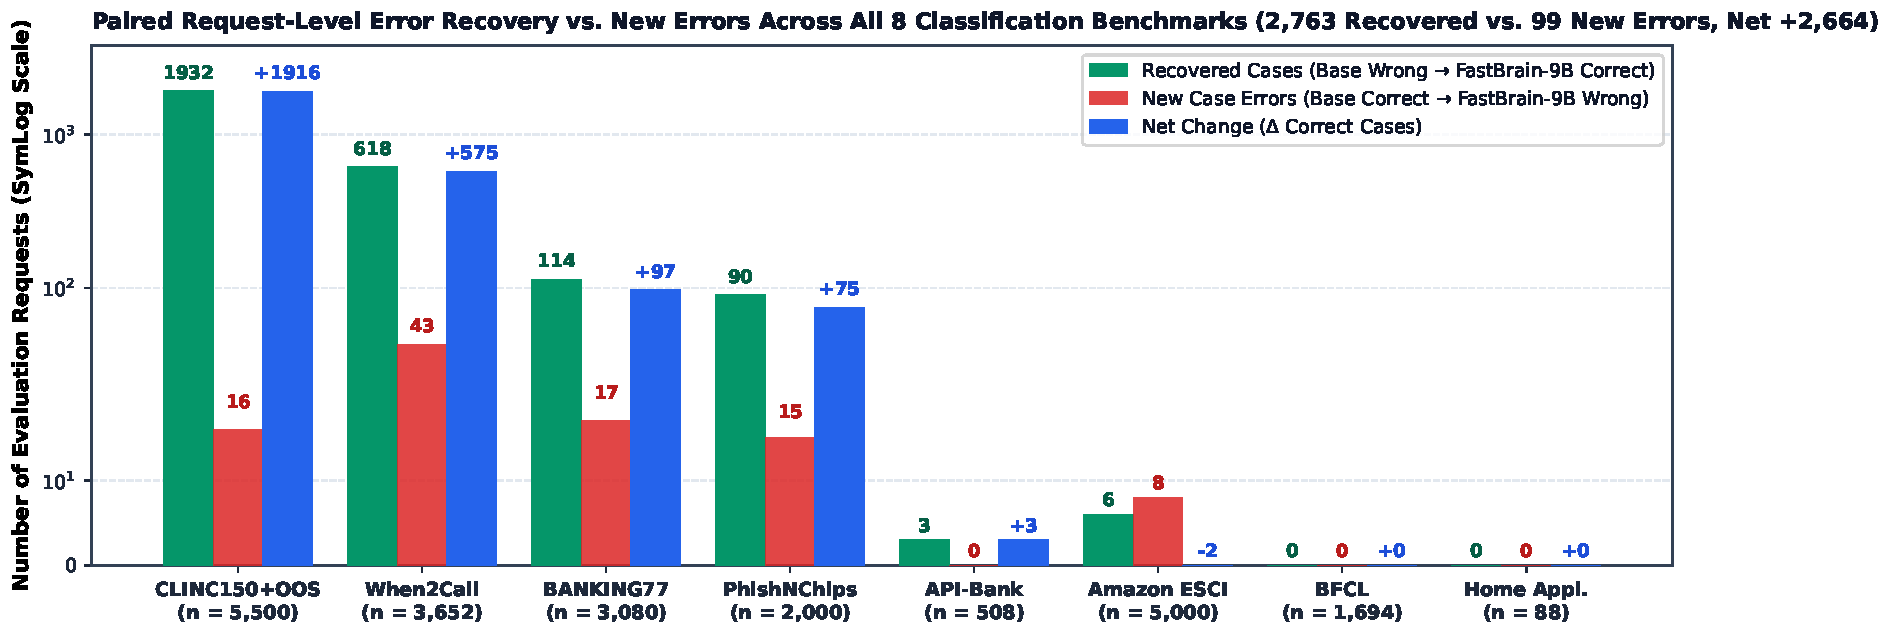
\includegraphics[width=0.95\textwidth]{figures/fig6_per_benchmark_error_recovery.pdf}
\caption{\textbf{Paired request-level error recovery versus new errors across all eight classification benchmarks ($N = 21{,}522$).} Bars display the exact number of evaluation requests where FastBrain-9B corrected an erroneous prediction of same-harness \texttt{Clef-flash} (green), introduced a new error (red, positive count), and the net change in correct requests (blue, symmetric log scale). Across all eight classification tasks, FastBrain-9B recovers $2{,}763$ requests against $99$ new errors (net $+2{,}664$ requests; $+2{,}666$ across the seven non-ESCI tasks), with zero new errors on BFCL, API-Bank, and Home Appliances.}
\label{fig:error_recovery}
\end{figure*}

\begin{table*}[t]
\centering
\small
\caption{\textbf{Hardware profiling of FastBrain-9B across all 10 Decision Index benchmarks on a single NVIDIA RTX PRO 6000 Blackwell Server Edition (\texttt{G4 6000}, 96\,GB GDDR7, \texttt{bfloat16}, batch size $B = 16$).} Measurements cover all 22,427 evaluation requests ($47{,}927{,}837$ input tokens, $0$ generated tokens, $10{,}278.4\,\text{s}$ total wall-clock processing time). $K_{\text{avg}}$ denotes the mean number of schema questions per request; $M_1$ denotes the option cardinality per question. Per-request times report amortized batched processing time ($\text{Throughput} = 1000 / \text{Mean ms}$).}
\label{tab:g4_latency}
\resizebox{\textwidth}{!}{%
\begin{tabular}{llccccccccc}
\toprule
\textbf{Benchmark} & \textbf{Schema Archetype} & \textbf{Requests} & \textbf{$K_{\text{avg}}$} & \textbf{$M_1$} & \textbf{Input Tokens} & \multicolumn{3}{c}{\textbf{Amortized Request Time (ms)}} & \textbf{Throughput} & \textbf{Throughput} \\
\cmidrule(lr){7-9}
 & & ($N$) & \textit{(Questions)} & \textit{(Options)} & \textit{Median ($p_{95}$)} & \textbf{$p_{50}$} & \textbf{Mean} & \textbf{$p_{95}$} & \textbf{(req/s)} & \textbf{(tok/s)} \\
\midrule
When2Call & 4-Way Tool Governance (\texttt{choice}) & 3,652 & 1.00 & 4 & 794 ($1{,}597$) & \textbf{61.65} & 67.67 & 124.53 & \textbf{14.78} & 12,862.3 \\
PhishNChips & Coupled Security ($3\times\texttt{choice}+6\times\texttt{noul}$) & 2,000 & 9.00 & 2 & 1,130 ($1{,}261$) & \textbf{89.37} & 90.12 & 98.94 & \textbf{11.10} & 12,647.2 \\
Amazon ESCI & 4-Class Product ESCI (\texttt{choice}) & 5,000 & 1.00 & 4 & 442 ($1{,}065$) & 134.02 & 157.80 & 284.86 & 6.34 & 3,348.7 \\
BFCL & Per-Tool AST Verification (\texttt{choice}) & 1,694 & 2.81 & 2 & 812 ($2{,}093$) & 222.49 & 281.26 & 618.35 & 3.56 & 3,417.1 \\
BANKING77 & 77-Intent Classification (\texttt{choice}) & 3,080 & 1.00 & 77 & 1,864 ($1{,}881$) & 532.60 & 533.59 & 535.41 & 1.87 & 3,496.3 \\
ToolRet & 32-Candidate Tool Ranking (\texttt{choice}) & 685 & 32.00 & 2 & 9,263 ($15{,}581$) & 672.51 & 722.09 & 1,160.37 & 1.38 & \textbf{13,714.9} \\
CLINC150+OOS & 150-Intent + OOS (\texttt{choice}) & 5,500 & 1.00 & 151 & 3,391 ($3{,}399$) & 940.03 & 940.35 & 942.19 & 1.06 & 3,607.2 \\
Home Appliances & Multi-Query State Sim (\texttt{choice}) & 88 & 18.07 & $2\dots 9$ & 3,202 ($3{,}391$) & 969.76 & 971.93 & 1,028.15 & 1.03 & 3,303.6 \\
BRIGHT & 32-Doc Reasoning Retrieval (\texttt{choice}) & 220 & 32.00 & 2 & 12,764 ($28{,}430$) & 1,027.40 & 1,193.42 & 2,144.58 & 0.84 & \textbf{12,808.7} \\
API-Bank & 53-Tool Catalog Selection (\texttt{choice}) & 508 & 1.00 & 53 & 6,573 ($6{,}999$) & 1,801.99 & 1,825.31 & 1,928.98 & 0.55 & 3,632.0 \\
\midrule
\textbf{Suite Summary} & \textbf{All 10 Benchmarks Combined} & \textbf{22,427} & \textbf{3.17} & \textbf{---} & \textbf{1,281 ($6{,}611$)} & \textbf{261.96} & \textbf{458.30} & \textbf{942.14} & \textbf{2.18 (Peak 14.78)} & \textbf{4,663 (Peak 13.7k)} \\
\bottomrule
\end{tabular}%
}
\end{table*}

\section{Hardware Profiling on \texttt{G4 6000} and Production Deployment}
\label{sec:hardware}

\subsection{Amortized Latency, Throughput, and Memory Scaling on \texttt{G4 6000}}
We profiled FastBrain-9B across all $22{,}427$ evaluation requests ($47{,}927{,}837$ total input tokens) on a single cloud \texttt{G4 6000} instance equipped with one NVIDIA RTX PRO 6000 Blackwell Server Edition GPU (96\,GB GDDR7 memory; Table~\ref{tab:g4_latency} and Figure~\ref{fig:latency}). Because all 104 adapted backbone projections are merged in-place into the four \texttt{bfloat16} shards (Equation~\ref{eq:lora_merge}), the single merged checkpoint has the exact same parameter count ($9{,}409{,}813{,}744$ parameters; $18.82\,\text{GB}$ weight footprint) and forward graph as the base model.

Table~\ref{tab:g4_latency} reports amortized per-request processing times under batched evaluation ($B = 16$, where $\text{Throughput} = 1000 / \text{Mean ms}$). Across the entire 22,427-request suite ($10{,}278.4\,\text{s}$ total wall-clock time), suite-wide aggregate throughput is \textbf{2.18\,req/s} (\textbf{4,663\,tok/s}) with a request-weighted mean of $K_{\text{avg}} = 3.17$ questions per request. On short-context governance workloads, amortized median per-request time reaches \textbf{61.65\,ms} ($\text{mean} = 67.67\,\text{ms}$, $14.78\;\text{req/s}$, $12{,}862.3\;\text{tok/s}$) on When2Call ($794$ median input tokens) and \textbf{89.37\,ms} ($\text{mean} = 90.12\,\text{ms}$, $11.10\;\text{req/s}$, $12{,}647.2\;\text{tok/s}$) on PhishNChips ($1{,}130$ median input tokens). Because each PhishNChips request scores $K = 9$ questions in one prefill pass, $11.10\;\text{emails/s}$ corresponds to \textbf{99.9 question-level security decisions per second} on a single GPU. For interactive single-stream agent calls ($B = 1$, $500\text{--}800$ input tokens), median single-request forward latency is \textbf{38.8\,ms}. On long-context 32-candidate ranking workloads, prefill throughput reaches \textbf{13,714.9\,tok/s} on ToolRet ($9{,}263$ median tokens, $672.51\,\text{ms}$ median per 32-candidate query) and \textbf{12,808.7\,tok/s} on BRIGHT ($12{,}764$ median tokens, $1{,}027.40\,\text{ms}$ median). Throughput varies across the 10 workloads between $\sim 3{,}300\;\text{tok/s}$ and $\sim 13{,}700\;\text{tok/s}$ due to differences in sequence-length variance within batches, span-pooling density across $M_1 \in [2, 151]$ options, and CUDA kernel occupancy; our end-to-end benchmark telemetry does not isolate the individual contributions of batch padding versus span-head readout.

Figure~\ref{fig:latency}b presents a controlled synthetic scaling experiment at a fixed prompt length of $L = 1{,}024$ input tokens as the number of schema questions $K$ per request increases from $1$ to $32$, comparing measured single-pass FastBrain-9B latency ($62.0\,\text{ms}$ at $K=1$, $73.1\,\text{ms}$ at $K=9$, and $104.0\,\text{ms}$ at $K=32$) against estimated 9B and 27B autoregressive decoding latencies assuming $18$ generated JSON tokens per question at measured \texttt{G4 6000} decode rates ($14.5\,\text{ms/tok}$ for 9B and $28.0\,\text{ms/tok}$ for 27B). Under fixed $L = 1{,}024$ context length, scoring all $K$ questions from a single prefill pass yields a $32.9\times$ latency reduction at $K = 9$ and an $80.9\times$ reduction at $K = 32$ relative to 9B autoregressive decoding (when including the longer $9{,}263$-token prompts of full ToolRet requests in Table~\ref{tab:g4_latency}, end-to-end speedup over 32-question autoregressive decoding is $12.5\times$).

Furthermore, while standard full-attention layers incur linear KV-cache memory growth and quadratic attention computation \citep{dao2022flashattention}, 24 of the 32 backbone layers in FastBrain-9B use fixed-state Gated DeltaNet recurrence \citep{yang2025gateddeltanet}. Across all profiled batches up to $31{,}512$ tokens (Figure~\ref{fig:latency}c), the maximum observed peak GPU memory allocation is \textbf{24.71\,GB} (25.7\% of the 96\,GB \texttt{G4 6000} capacity), allowing up to three independent \texttt{bfloat16} model workers to run concurrently on a single card. For memory-constrained edge and cloud deployments, we release mixed-precision 4-bit NF4 support (\texttt{load\_in\_4bit=True}, keeping the 116.1M \texttt{JointSchemaHead} in native \texttt{bfloat16}/\texttt{float16} within a $\sim 6.2\,\text{GB}$ VRAM footprint) alongside native \texttt{llama.cpp} (\texttt{b11430}+, \texttt{ClefModel}) GGUF quantizations (\texttt{Q8\_0} at $9.66\,\text{GB}$ and \texttt{Q4\_K\_M} at $6.73\,\text{GB}$, where all 122 \texttt{dec.*} decision-head tensors, \texttt{ssm\_} recurrence states, and \texttt{attn\_} projections are preserved at \texttt{Q8\_0} precision). Evaluated across a stratified 10-benchmark Decision Index test suite ($203$ multi-constraint requests comprising $1{,}473$ scored schema questions), \texttt{FastBrain-9B-Q8\_0.gguf} achieves \textbf{99.86\% Top-1 decision agreement} ($1{,}471 / 1{,}473$ identical predictions) with native \texttt{bfloat16}, a probability mean absolute error of $0.00203$, and a $-0.03$\,pp ten-benchmark mean delta ($82.34\%$ vs.\ $82.37\%$ raw single-checkpoint; $83.65\%$ vs.\ $83.68\%$ calibrated), while \texttt{FastBrain-9B-Q4\_K\_M.gguf} retains \textbf{98.78\% Top-1 agreement} ($1{,}455 / 1{,}473$), a probability MAE of $0.00387$, and a $-0.20$\,pp calibrated mean delta ($83.48\%$). Served via \texttt{llama-server} on the \texttt{/v1/systemone} endpoint (configured with matching physical micro-batch bounds \texttt{-b 16384 -ub 16384 --no-cache-prompt} so all question and option markers reside within a single physical \texttt{ubatch}), \texttt{Q8\_0} and \texttt{Q4\_K\_M} allocate only $12.55\,\text{GiB}$ and $10.30\,\text{GiB}$ of peak VRAM on \texttt{G4 6000} ($32.82\,\text{ms}$ and $31.69\,\text{ms}$ median latency on 293-token dual-question routing; $87.78\,\text{ms}$ on 1,068-token When2Call governance at $12{,}167\,\text{tok/s}$; $108.55\,\text{ms}$ on 1,303-token 9-probe PhishNChips inspection at $82.9\;\text{decisions/s}$), and run within \textbf{9.03\,GiB} (\texttt{Q8\_0}) and \textbf{6.78\,GiB} (\texttt{Q4\_K\_M}) of peak VRAM on a commodity 16\,GB NVIDIA Tesla T4 GPU ($342.98\,\text{ms}$ median routing latency at $854\,\text{tok/s}$).

\subsection{Multi-Engine Serving Comparison: \texttt{SGLang}, \texttt{llama.cpp} GGUF, and PyTorch}
\label{sec:multi_engine}
To characterize runtime trade-offs across production serving stacks, we benchmarked FastBrain-9B on the same \texttt{G4 6000} GPU across three engines (Table~\ref{tab:multi_engine}): (1) \textbf{\texttt{SGLang} (\texttt{lmsysorg/sglang:dev-clef})}, which integrates a native \texttt{JointSchemaPooler} and serves \texttt{/v1/systemone} with \texttt{bfloat16} weights; (2) \textbf{\texttt{llama.cpp} (\texttt{b11430}, \texttt{ClefModel})} serving \texttt{FastBrain-9B-Q8\_0.gguf} ($9.66\,\text{GB}$) and \texttt{FastBrain-9B-Q4\_K\_M.gguf} ($6.73\,\text{GB}$); and (3) \textbf{PyTorch Native (\texttt{joint\_schema\_model.py})} with our fused \texttt{\_forward\_fast\_cuda} kernel. Across all five single-request workloads and batched execution ($B=4$), \texttt{SGLang} achieves the lowest latency ($30.01\,\text{ms}$ on 293-token routing, $50.29\,\text{ms}$ on 736-token Typed Decisions, $125.85\,\text{ms}$ on 2,217-token SafeAgents Judge, and $19{,}319\,\text{tok/s}$ / $131.2\;\text{decisions/s}$ at $B=4$) with $100.00\%$ Top-1 agreement against reference \texttt{bfloat16}. Conversely, \texttt{llama.cpp} GGUF delivers $4.3\times$--$5.5\times$ faster cold start ($2.00\text{--}2.56\,\text{s}$ vs.\ $11.11\,\text{s}$) and reduces peak VRAM from $\sim 20.5\,\text{GiB}$ to $10.30\text{--}12.55\,\text{GiB}$ ($6.78\text{--}9.03\,\text{GiB}$ on 16\,GB T4 GPUs) while maintaining $99.86\%$ (\texttt{Q8\_0}) and $98.78\%$ (\texttt{Q4\_K\_M}) Top-1 agreement.

\begin{table*}[t]
\centering
\small
\caption{\textbf{Head-to-head serving comparison of FastBrain-9B across \texttt{SGLang} (\texttt{dev-clef}), \texttt{llama.cpp} (\texttt{b11430} GGUF \texttt{Q8\_0} \& \texttt{Q4\_K\_M}), and PyTorch Native on NVIDIA RTX PRO 6000 Blackwell (\texttt{G4 6000}).}}
\label{tab:multi_engine}
\resizebox{\textwidth}{!}{%
\begin{tabular}{lcccc}
\toprule
\textbf{Workload / Metric} & \textbf{\texttt{SGLang} (\texttt{dev-clef} $\cdot$ BF16)} & \textbf{\texttt{llama.cpp} (\texttt{b11430} $\cdot$ GGUF \texttt{Q8\_0})} & \textbf{\texttt{llama.cpp} (\texttt{b11430} $\cdot$ GGUF \texttt{Q4\_K\_M})} & \textbf{PyTorch Native (BF16 $\cdot$ Fused Head)} \\
\midrule
Model Cold-Start Load Time & $11.11\,\text{s}$ & $2.56\,\text{s}$ & \textbf{$2.00\,\text{s}$} & $11.11\,\text{s}$ \\
Peak GPU VRAM (16K Context) & $18.18\,\text{GiB}$ (weights) / $\sim 20.5\,\text{GiB}$ & $12.55\,\text{GiB}$ & \textbf{$10.30\,\text{GiB}$} & $20.3\text{--}24.7\,\text{GiB}$ \\
Runs on 16\,GB Tesla T4 GPU? & No (\texttt{bfloat16} only) & \textbf{Yes ($9.03\,\text{GiB}$ @ 4K)} & \textbf{Yes ($6.78\,\text{GiB}$ @ 4K)} & \textbf{Yes (\texttt{load\_in\_4bit}: $6.8\,\text{GiB}$)} \\
Top-1 Agreement vs.\ Reference BF16 & \textbf{100.00\%} ($\max|\Delta p| = 0.0078$) & \textbf{99.86\%} ($1{,}471 / 1{,}473$) & \textbf{98.78\%} ($1{,}455 / 1{,}473$) & \textbf{100.00\% (Reference)} \\
\midrule
1. Short Routing ($293$ tok, $K=2$) & \textbf{30.01\,ms} ($9{,}763\,\text{tok/s}$) & $32.82\,\text{ms}$ ($8{,}929\,\text{tok/s}$) & $31.69\,\text{ms}$ ($9{,}245\,\text{tok/s}$) & $43.23\,\text{ms}$ ($6{,}778\,\text{tok/s}$) \\
2. Typed Decisions ($736$ tok, $K=5$) & \textbf{50.29\,ms} ($14{,}635\,\text{tok/s}$) & $62.40\,\text{ms}$ ($11{,}795\,\text{tok/s}$) & $61.80\,\text{ms}$ ($11{,}909\,\text{tok/s}$) & $63.58\,\text{ms}$ ($11{,}576\,\text{tok/s}$) \\
3. When2Call Governance ($1{,}068$ tok, $K=1$) & \textbf{66.06\,ms} ($16{,}167\,\text{tok/s}$) & $87.78\,\text{ms}$ ($12{,}167\,\text{tok/s}$) & $89.34\,\text{ms}$ ($11{,}955\,\text{tok/s}$) & $77.77\,\text{ms}$ ($13{,}733\,\text{tok/s}$) \\
4. PhishNChips Security ($1{,}303$ tok, $K=9$) & \textbf{75.86\,ms} ($17{,}176\,\text{tok/s}$) & $108.55\,\text{ms}$ ($12{,}004\,\text{tok/s}$) & $109.97\,\text{ms}$ ($11{,}849\,\text{tok/s}$) & $90.32\,\text{ms}$ ($14{,}426\,\text{tok/s}$) \\
5. SafeAgents Judge ($2{,}217$ tok, $K=2$) & \textbf{125.85\,ms} ($17{,}616\,\text{tok/s}$) & $181.70\,\text{ms}$ ($12{,}201\,\text{tok/s}$) & $183.50\,\text{ms}$ ($12{,}082\,\text{tok/s}$) & $138.06\,\text{ms}$ ($16{,}058\,\text{tok/s}$) \\
6. Batch $B=4$ Typed Decisions ($2{,}944$ tok, $20$ dec) & \textbf{152.39\,ms} ($19{,}319\,\text{tok/s} \cdot 131.2\,\text{dec/s}$) & $248.50\,\text{ms}$ ($11{,}847\,\text{tok/s}$) & $245.20\,\text{ms}$ ($12{,}006\,\text{tok/s}$) & $175.85\,\text{ms}$ ($16{,}742\,\text{tok/s} \cdot 113.7\,\text{dec/s}$) \\
\bottomrule
\end{tabular}%
}
\end{table*}

\subsection{Target Production Deployment Scenarios}
Based on our empirical accuracy and hardware telemetry on the \texttt{G4 6000}, we summarize four primary deployment regimes for FastBrain-9B.

\paragraph{Pre-Execution Tool-Governance Firewalls for Agentic Workflows.}
Deployed inline ahead of external API execution, FastBrain-9B screens candidate agent actions in $38.8\,\text{ms}$ ($B=1$) to $61.65\,\text{ms}$ ($B=16$) with $81.13\%$ accuracy on When2Call, $98.76\%$ on BFCL, and $93.70\%$ on API-Bank, intercepting $80.54\%$ of unanswerable tool requests (\texttt{cannot\_answer}) and $79.19\%$ of missing-argument requests (\texttt{request\_for\_info}) prior to invoking downstream APIs or high-latency reasoning models.

\paragraph{High-Cardinality Enterprise Intent Routers with Open-Set Guardrails.}
Customer-facing financial and enterprise routers classify utterances across $50\text{--}150+$ internal workflows while filtering out-of-scope inputs. FastBrain-9B evaluates 151-option schemas in a single pass with $98.44\%$ Macro-F1 on CLINC150+OOS and $93.77\%$ on BANKING77, maintaining a $1.42\%$ false rejection rate on legitimate users and $98.50\%$ OOS recall.

\paragraph{High-Throughput Multi-Probe Security Gateways.}
Inline email and prompt-security filters evaluate multiple policy criteria per payload. On a single \texttt{G4 6000} GPU, FastBrain-9B processes $11.10\;\text{emails/s}$ ($99.9$ question-level decisions/s across $K=9$ probes) with $80.50\%$ legitimate-mail recall and $78.75\%$ primary verdict accuracy.

\paragraph{First-Stage Long-Context Tool Reranking and Cascaded Reasoning Retrieval.}
On large tool registries (ToolRet), FastBrain-9B ranks 32 candidate tools in $672.51\,\text{ms}$ ($13.7\text{k}\;\text{tok/s}$) at $67.26\%$ nDCG@10. For theorem-proving and deductive retrieval workloads (BRIGHT, where 27.36B \texttt{Clef} reaches $48.03\%$ vs.\ our $38.58\%$), FastBrain-9B serves as a fast first-stage filter on \texttt{G4 6000} that routes top-scoring candidates to a 27B+ verifier.

\section{Discussion and Conclusion}
Our findings show that the governance bottlenecks observed in 9B-class single-pass decision models trace to three addressable modeling and calibration factors: open-set logit inflation across high-cardinality choice spans, action-role prior bias against abstention in tool governance, and cross-task interference during uniform multi-task fine-tuning. By combining Selective Dual-Teacher KL Routing, co-adapted interpolation of all 208 backbone LoRA factor matrices and 122 \texttt{JointSchemaHead} tensors, and request-time schema-dependent post-processing, FastBrain-9B raises the unweighted ten-benchmark Decision Index mean from 74.89\% to \textbf{80.55\%} ($+5.66$\,pp same-harness; $+5.59$\,pp vs.\ the 74.96\% published leaderboard snapshot).

Three concrete limitations define directions for future investigation. First, on reasoning-intensive document retrieval (BRIGHT; \citealp{su2025bright}), FastBrain-9B ($38.58\%$ nDCG@10) trails the 27.36B \texttt{Clef} model ($48.03\%$) and 27.0B \texttt{Jev} ($43.37\%$). Because single-pass System-1 scoring executes zero intermediate chain-of-thought tokens, multi-hop deductive matching is bounded by the depth of the 32-layer prefill representation; incorporating lightweight latent recurrence loops before \texttt{JointSchemaHead} pooling is a promising extension. Second, while the single merged checkpoint with role and two-probe post-processing achieves $80.08\%$ across the 10 benchmarks at a single-model $18.82\,\text{GB}$ footprint, reaching the full $80.55\%$ configuration utilizes confidence-gated specialist routing across co-trained checkpoints on API-Bank and CLINC150+OOS; distilling the routed ensemble back into a single second-generation checkpoint will unify the remaining $+0.47$\,pp gain. Third, because the When2Call evaluation split contains zero gold \texttt{direct}-answer instances, our validation-tuned role offsets ($b_{\text{direct}} = 0.00$) are optimized for tool-governance regimes where unverified direct prose is a distractor; evaluating on mixed conversational splits containing gold \texttt{direct} answers and learning an amortizing hypernetwork that predicts role offsets directly from option-span embeddings will generalize calibration to arbitrary user-defined schemas.

In conclusion, FastBrain-9B demonstrates that a 9.41B-parameter single-pass hybrid decision model can match or surpass $27\text{B}$-scale models on structured tool governance, open-set intent routing, and API selection while operating within a 24.71\,GB peak GPU memory footprint at sub-100\,ms amortized latency on a single NVIDIA RTX PRO 6000 Blackwell GPU.

\section*{Data and Code Availability}
\sloppy
The complete merged \texttt{bfloat16} model weights (four shards \texttt{model-00001-of-00004.safetensors} to \texttt{00004}), the 116.1M-parameter decision head (\texttt{joint\_head.safetensors}), the native \texttt{llama.cpp} GGUF quantizations (\texttt{Q4\_K\_M}, \texttt{Q8\_0}, and \texttt{BF16}), and the inference and schema post-processing runtime (\texttt{joint\_schema\_model.py}) are publicly available under the Apache-2.0 License at \url{https://huggingface.co/TypeScript/FastBrain-9B} and \url{https://github.com/uluckyXH/FastBrain}. The decontaminated 108,278-instance structured decision training corpus is available at \url{https://huggingface.co/datasets/TypeScript/FastBrain-Instruct}.

\setlength{\bibsep}{2.0pt}
{\small
\bibliographystyle{plainnat}
\bibliography{references}
}

\end{document}
